\chapter{Results and Discussion}
\section{Baseline performance of the forecasting models}
In this study, five machine learning algorithms were trained with univariate datasets to predict the ammonia concentrations and colour levels in the reclaimed water system. All baseline models are trained by training datasets which were not applied with data pre-processing and feature engineering techniques. The forecasting model performance is presented in Fig.~\ref{fig:baseline-performance}. As shown in Fig.~\ref{fig:baseline-nh3}, the test loss values of RF, DNN, RNN, GRU, and LSTM models are 0.1158, 0.0561, 0.0440, 0.0414, and 0.0405, respectively. RF model is the least capable model in forecasting ammonia concentrations, given that its test loss is significantly higher than all the other four deep learning models. The cause of poor RF model performance can be attributed to its simple model structure. RF model generates results based on the averaging results from each decision tree (i.e., each decision tree will generate a prediction based on entropy and information gain). There is only one available hyperparameter for tuning RF models: the estimators (i.e., the number of the decision tree). Therefore, throughout the entire model tuning process. We observed the RF model had the lowest test loss at the beginning among all the models, and the increased estimators did not help lower the test loss values. Meanwhile, several iterations of hyperparameter tunings help the deep learning models to reduce the test loss values to critical values, which were lower than the test loss of the RF model. The gradual reductions of test loss values for deep learning models can be attributed to the nature of their complex model architectures (i.e., a good quantity of neurons, neurons are designed to perform unique functions) and the available hyperparameters for tuning. For instance, the number of hidden layers, number of neurons, learning rate, and epoch are adjustable. The customizable hyperparameters in the deep learning models allow the researchers to fully explore the possibilities of training better models, and the superior performance is reflected in the values of test loss obtained from the optimized hyperparameter settings.
%RF is the least capable model, complexity of model architecture, 
\begin{figure}[!ht]
  \centering
  \begin{subfigure}[t]{0.75\textwidth}
    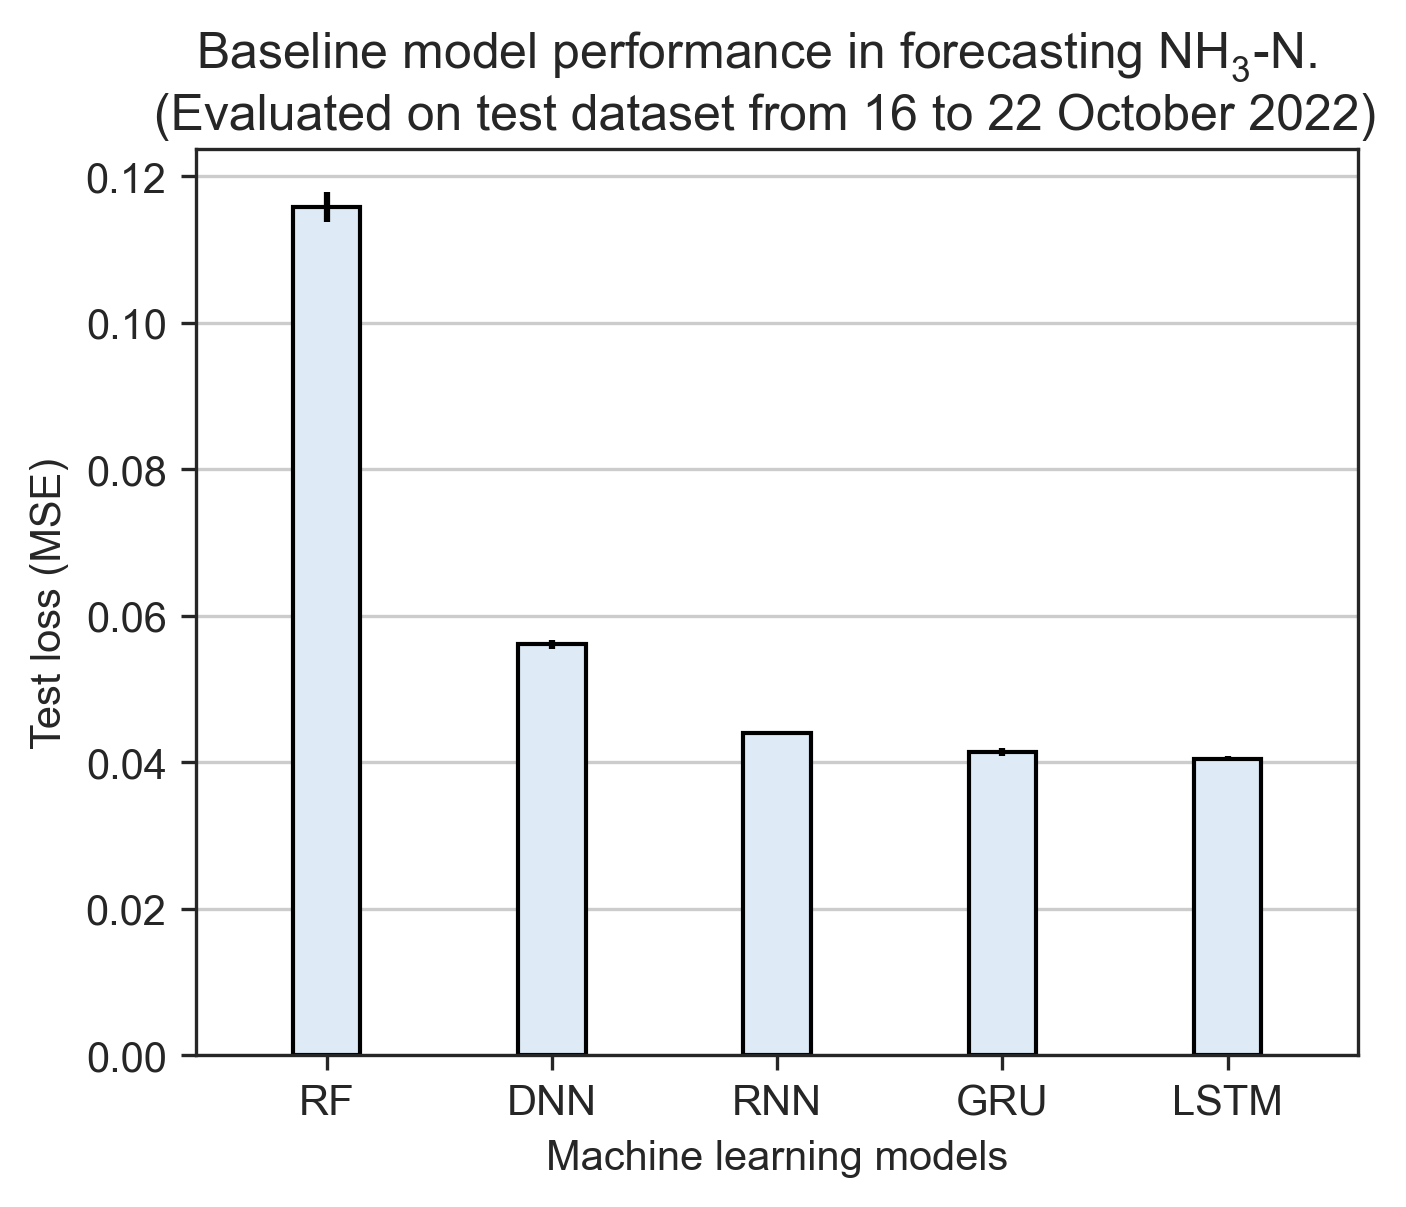
\includegraphics[width=\linewidth]{imgs/results/baseline-models-nh3.png}
    \caption{Test loss values from five ammonia forecasting models.} \label{fig:baseline-nh3}
  \end{subfigure}\\
  \vspace{2em}%   % maximize separation between the subfigures
  \begin{subfigure}[t]{0.75\textwidth}
    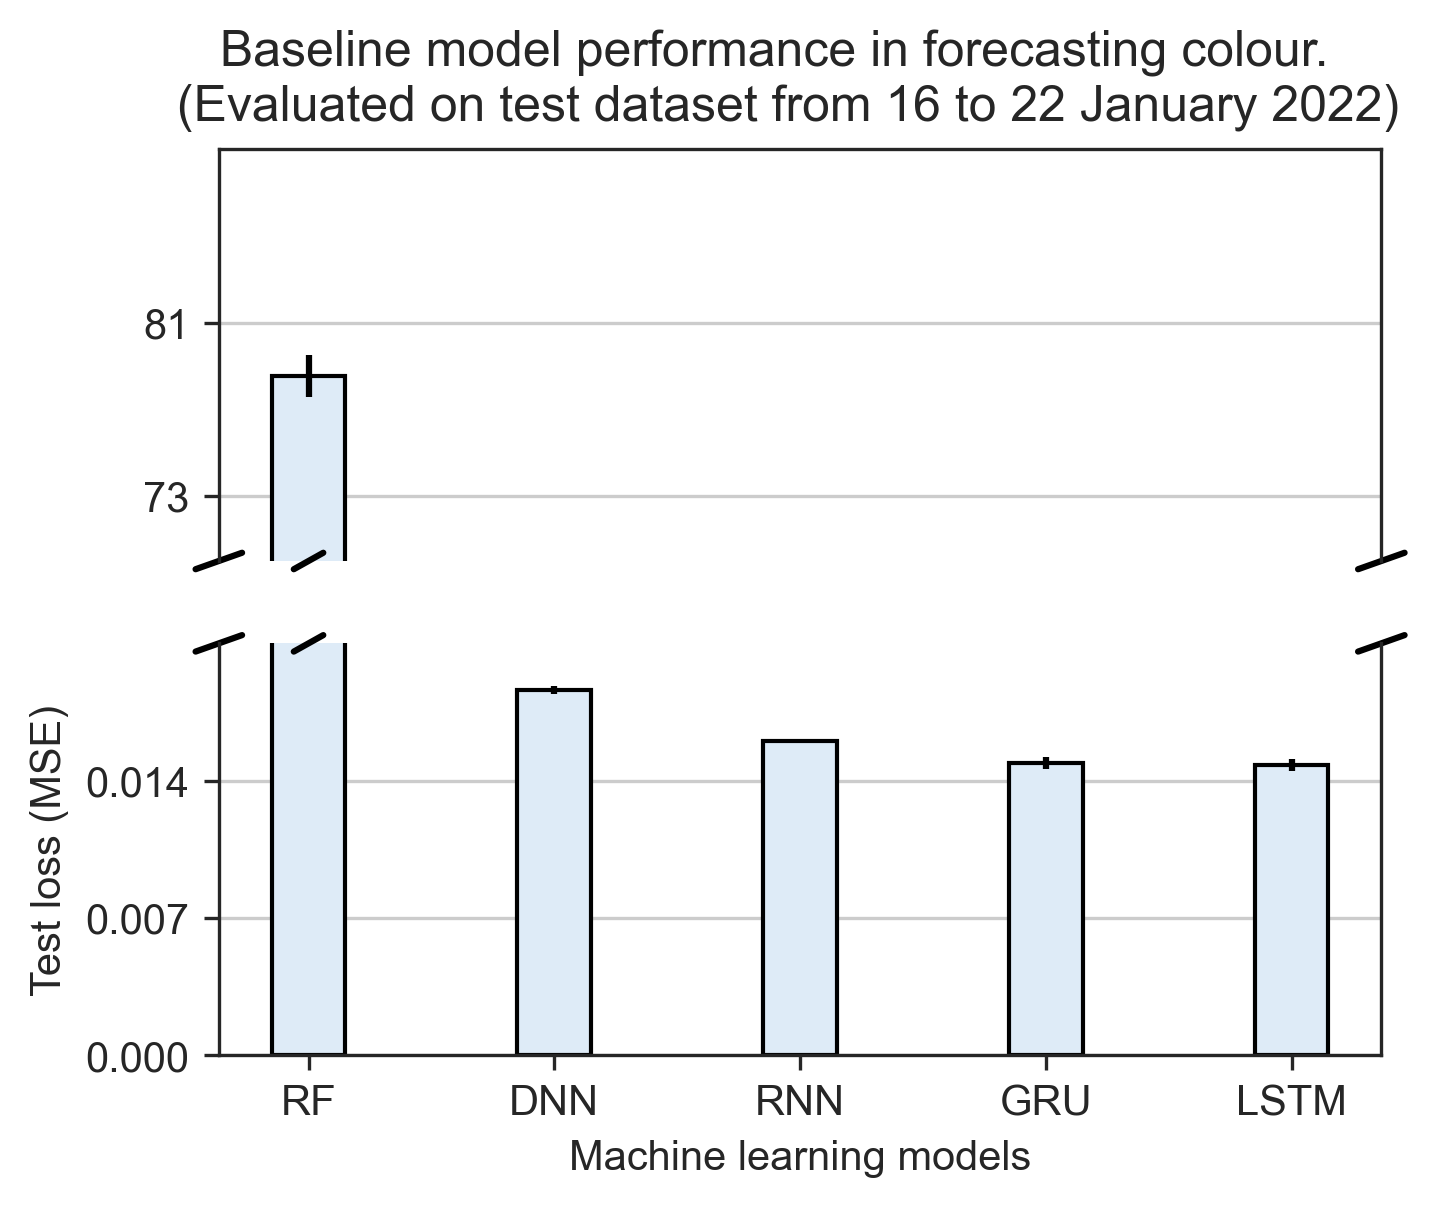
\includegraphics[width=\linewidth]{imgs/results/baseline-models-colour.png}
    \caption{Test loss values from five colour forecasting models.} \label{fig:baseline-colour}
  \end{subfigure}\\
\caption{Baseline performance of ammonia and colour forecasting models.} \label{fig:baseline-performance}
\end{figure}

GRU and LSTM models learn the data in similar ways by utilizing memorizing cells to pass and receive critical information from the previous memorizing cells, known as the architecture of recurrent neural network. Compared to RNN models, both models contain more "gates" in the architectures to help control the flow of information, enabling the models to capture more details. The number of gates in RNN, GRU, and LSTM is one, three, and four; theoretically, GRU and LSTM can learn more information from the data based on a greater number of gates. The results in Fig.~\ref{fig:baseline-nh3} showed good agreement with our understanding that LSTM performed better than GRU, followed by RNN models based on the values of test loss. For DNN models, the lack of memorizing cells in the model architecture relates to the poorer capability of learning information hidden in time-series datasets. In other words, DNN models cannot comprehend the information hidden in each datapoint in sequence, making the time-series dataset merely a common set of data. The DNN model with a test loss of 0.0440, higher than the 0.0414 of the RNN models, fully justifies the need to use the architecture of recurrent neural networks for training ammonia forecasting models.
%The strength of memorizing cell from the recurrent neural network structure, making LSTM the best model.

In Fig.~\ref{fig:baseline-colour}, the test loss from colour forecasting models are 78.5296, 0.0186, 0.0160, 0.0149, and 0.0148 for RF, DNN, RNN, GRU and LSTM models, respectively. We first noticed the highest test loss value of 78.5296 in the RF model compared to the other four, making RF model the worst model in forecasting colour levels. The extremely high MSE values were caused by the colour levels fluctuating in a wider range of 80 to 160 Hazen Units. The large discrepancy between the actual and predicted colour levels increases the error values, which are further amplified as the MSE values are calculated by the average of the squares of the errors. As shown in Fig.~\ref{fig:baseline-colour-plot-rf}, on 20 January 2022, the errors between the ground truth and forecasted values are up to around 30 Hazen Units, which contribute to a large increase of MSE values in the test loss. RF model is regarded as an inferior model for forecasting colour levels using the data collected in SWHEPP.
%MSE, RF the poorest

The performance of DNN, RNN, GRU, and LSTM models, from the best to the least, are identical to what we observed in the results of ammonia forecasting models. LSTM model has the lowest test loss of 0.0148, followed by the GRU, RNN, and DNN models. In colour forecasting models, the model performance of LSTM is very close to GRU, with a difference of less than 0.0001 (i.e., less than 1\%). However, the lowest test loss generated from the LSTM model in all the experiment runs (i.e., three runs) is 0.0143, which is lower than 0.0146 from the GRU model. Indicating LSTM model has more potential in forecasting time-series data.
%LSTM is the best

The significantly higher test loss of RF models compared to other models can be visualized by plotting the forecasted values with the ground truths (i.e., observed values). In Fig.~\ref{fig:baseline-plot-ammonia} and Fig.~\ref{fig:baseline-plot-colour}, one-step-ahead forecast horizon of ammonia concentrations and colour levels are plotted by RF as in Fig.~\ref{fig:baseline-nh3-plot-rf} and Fig.~\ref{fig:baseline-colour-plot-rf} and LSTM models as in Fig.~\ref{fig:baseline-nh3-plot-lstm} and Fig.~\ref{fig:baseline-colour-plot-lstm}. It is easier to observe that the RF models are less capable of predicting the water quality parameters. 


\begin{figure}[!ht]
    \centering
    \begin{subfigure}[t]{0.75\textwidth}
      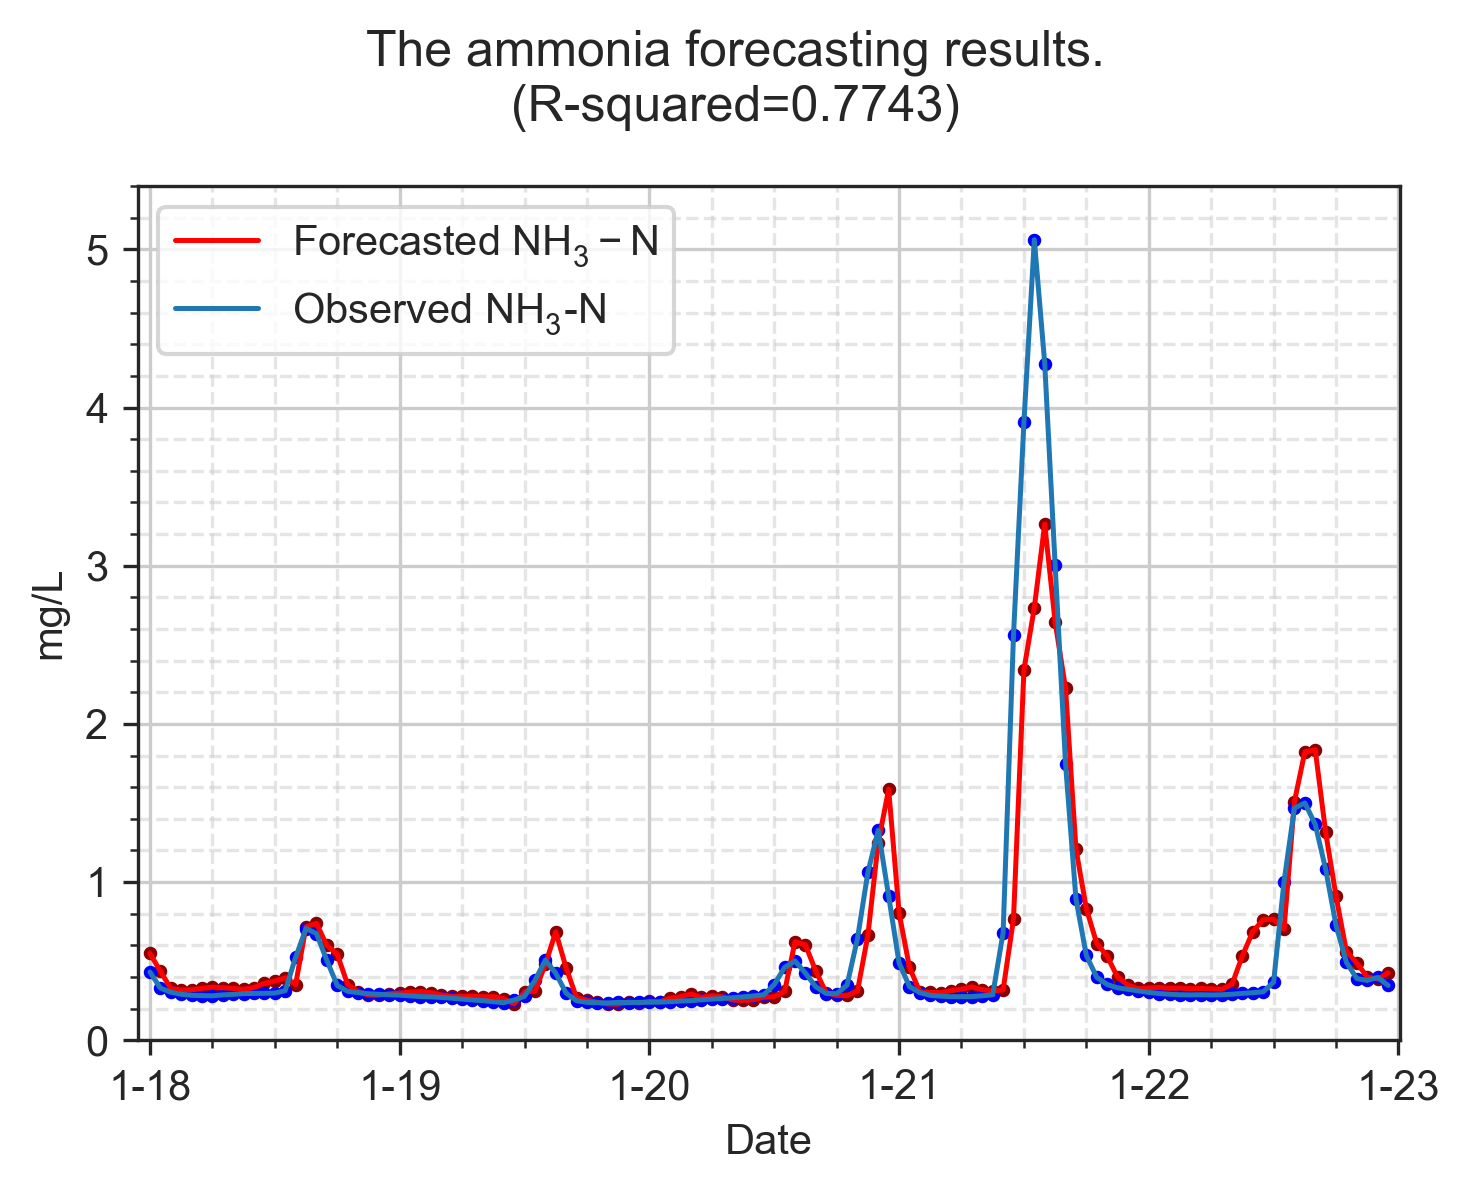
\includegraphics[width=\linewidth]{imgs/results/ammonia-colour-forecast-plot/00-RF_1_pred_Step1-obs-nh3.png}
      \caption{Baseline RF model forecasting ammonia concentration.} \label{fig:baseline-nh3-plot-rf}
    \end{subfigure}\\
    \vspace{1em}%   % maximize separation between the subfigures
    \begin{subfigure}[t]{0.75\textwidth}
      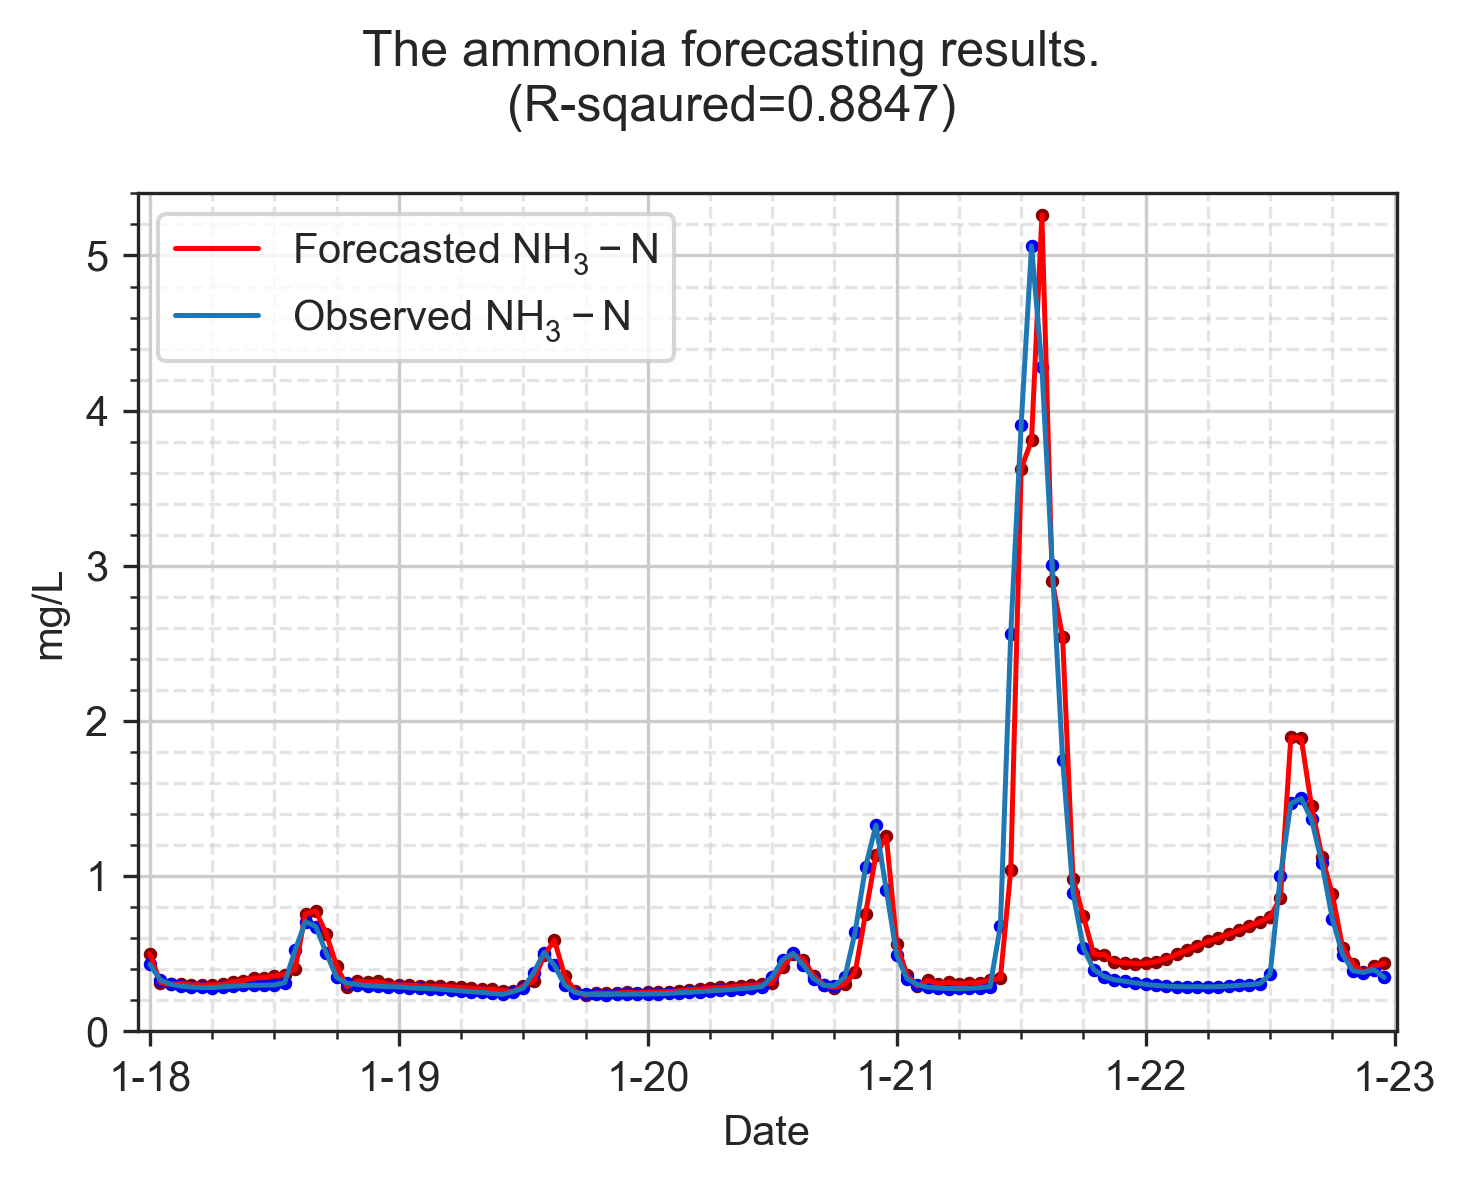
\includegraphics[width=\linewidth]{imgs/results/ammonia-colour-forecast-plot/00-LSTM_1_pred_Step1-obs-nh3.png}
      \caption{Baseline LSTM model forecasting ammonia concentration.} \label{fig:baseline-nh3-plot-lstm}
    \end{subfigure}\\
  \caption{Visulization of the model forecasting results.} \label{fig:baseline-plot-ammonia}
\end{figure}


\begin{figure}[!ht]
  \centering
    \begin{subfigure}[t]{0.75\textwidth}
      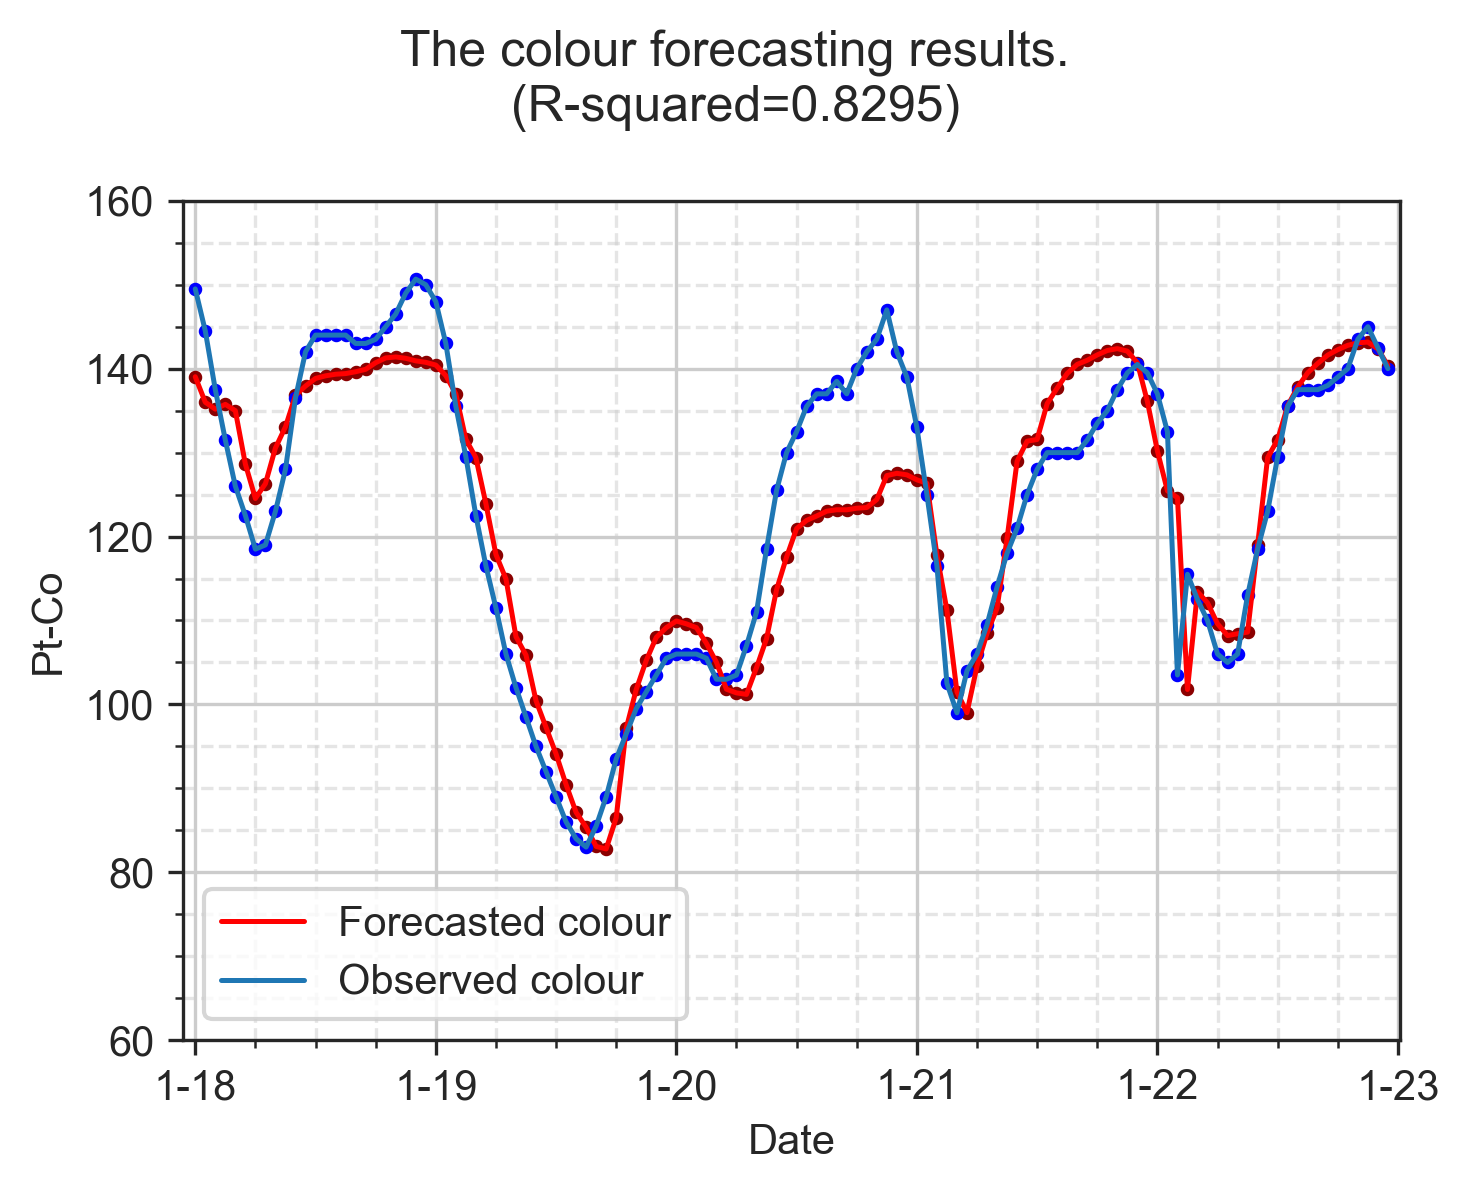
\includegraphics[width=\linewidth]{imgs/results/ammonia-colour-forecast-plot/00-RF_1_pred_Step1-obs-colour.png}
      \caption{Baseline RF model forecasting colour levels.} \label{fig:baseline-colour-plot-rf}
    \end{subfigure}\\ 
    \vspace{1em}%   % maximize separation between the subfigures
    \begin{subfigure}[t]{0.75\textwidth}
      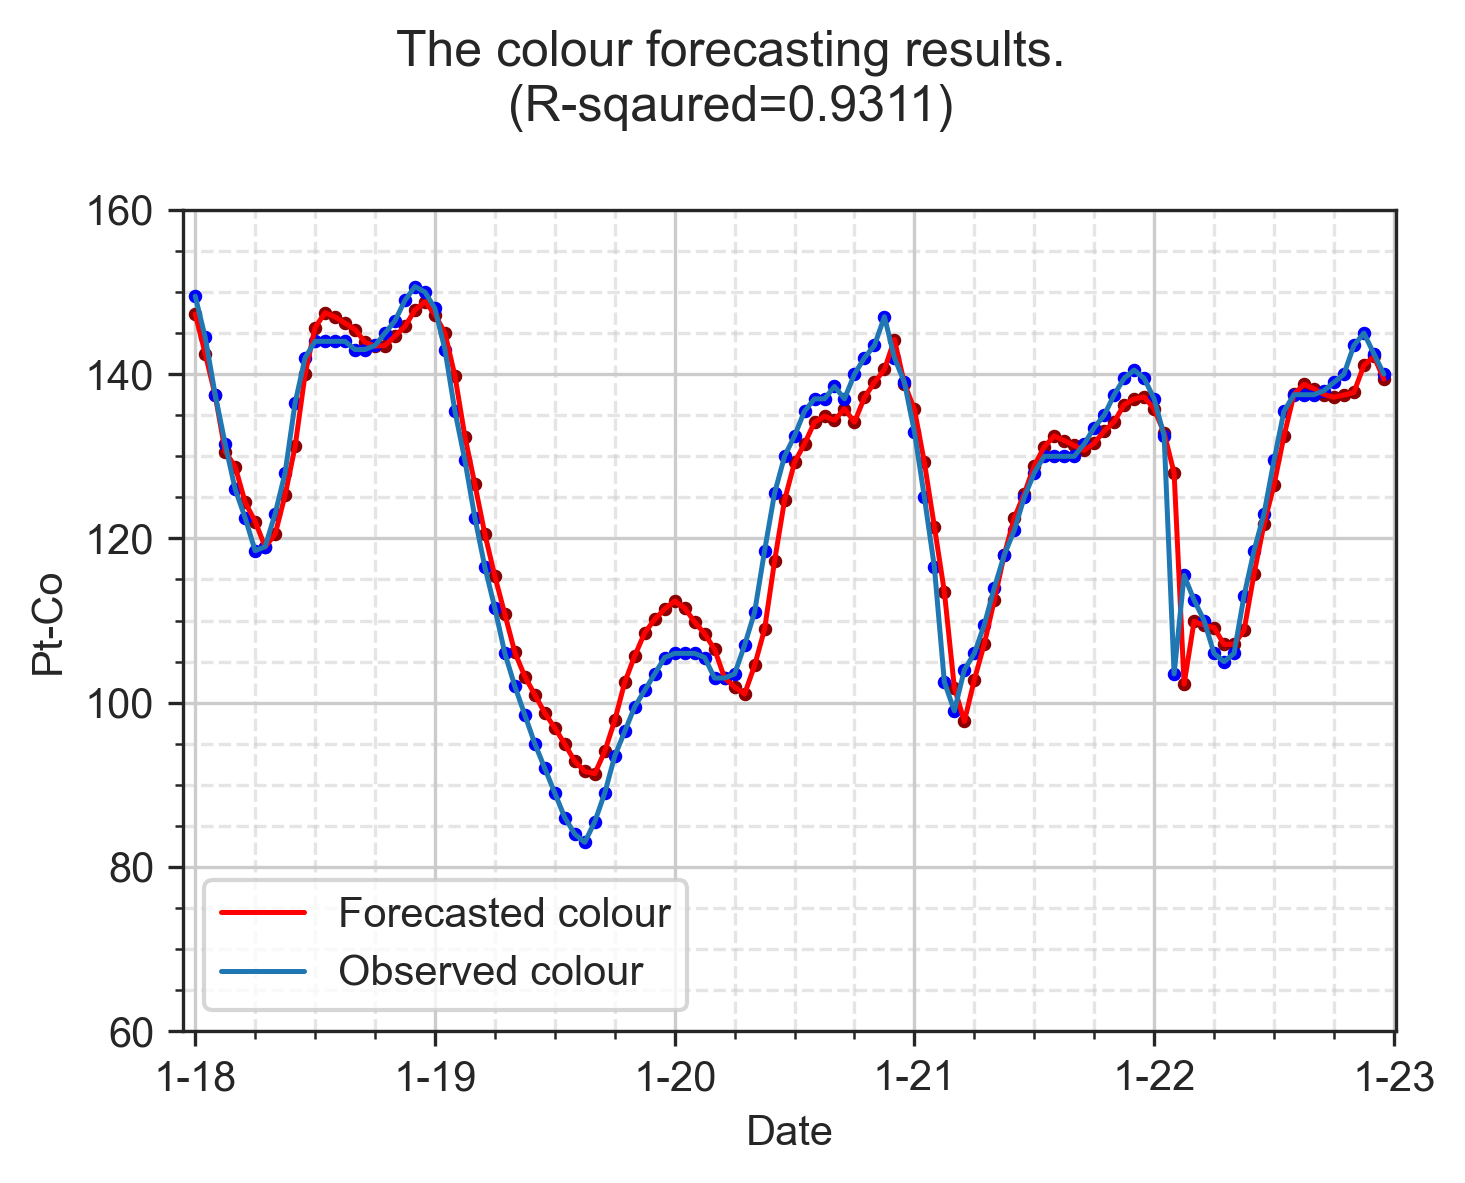
\includegraphics[width=\linewidth]{imgs/results/ammonia-colour-forecast-plot/00-LSTM_1_pred_Step1-obs-colour.png}
      \caption{Baseline LSTM model forecasting colour levels.} \label{fig:baseline-colour-plot-lstm}
    \end{subfigure}\\
  \caption{Visulization of the model forecasting results.} \label{fig:baseline-plot-colour}
\end{figure}

\section{Improved performance on forecasting models using data pre-processing techniques}
\subsection{Models trained by pre-processed datasets}

In this study, we investigate whether the datasets treated by the proposed data pre-processing techniques can improve the baseline model performance using the same hyperparameter settings. As shown in Table.~\ref{tab:baseline-result-jan-nh3} and Table.~\ref{tab:baseline-result-jan-colour}, we listed all the test loss values of five machine learning algorithms trained with each proposed pre-processed technique for ammonia concentrations and colour levels forecasting. The machine learning algorithm trained by datasets that were applied with SG filters at different window sizes is denoted as model-sg5, model-sg7, and model-sg9. The naming rule applies the same to EWMA filtered dataset; the method of outlier removal for ammonia data is denoted as model-or; models trained with the raw datasets are denoted as model-obs (i.e., observed dataset).

\begin{table}[!ht]
  \centering
  \caption{Baseline performance of ammonia forecasting model, evaluated on test dataset from \textbf{16 to 22 Janurary 2022}. Loss values are calculated by MSE.}\label{tab:baseline-result-jan-nh3}
  \begin{NiceTabular}{lcclcc}
      \toprule
      Model-Dataset & Test loss & Valid loss & Model-Dataset & Test loss & Valid loss \\
      \midrule
      GRU-sg7  & 0.0383 &1.2508&RNN-or  & 0.0432&1.6345 \\
      GRU-sg5  & 0.0385 &1.2644&RNN-ew3 & 0.0434&1.6041 \\
      LSTM-ew3 & 0.0388 &1.0796&RNN-obs & 0.0440&1.6734 \\
      LSTM-sg5 & 0.0388 &1.2346&RNN-sg9 & 0.0442&1.7046 \\
      LSTM-sg7 & 0.0388 &1.1804&DNN-obs & 0.0561&3.2383 \\
      GRU-ew2  & 0.0389 &1.1891&DNN-sg5 & 0.0562&3.2170 \\
      GRU-ew4  & 0.0391 &1.2390&DNN-ew2 & 0.0563&3.1677 \\
      GRU-ew3  & 0.0392 &1.2199&DNN-ew3 & 0.0569&3.2317 \\
      LSTM-ew2 & 0.0392 &1.0969&DNN-sg7 & 0.0570&3.2014 \\
      LSTM-ew4 & 0.0395 &1.1219&DNN-ew4 & 0.0571&3.2188 \\
      GRU-sg9  & 0.0396 &1.3097&DNN-or  & 0.0572&3.1972 \\
      LSTM-or  & 0.0398 &1.2612&DNN-sg9 & 0.0574&3.2484 \\
      LSTM-obs & 0.0405 &1.3993&RF-obs  & 0.1158&- \\
      GRU-or   & 0.0405 &1.2366&RF-sg9  & 0.1196&- \\
      LSTM-sg9 & 0.0410 &1.3076&RF-ew2  & 0.1286&- \\
      GRU-obs  & 0.0414 &1.3638&RF-or   & 0.1294&- \\
      RNN-sg5  & 0.0415 &1.5088&RF-sg5  & 0.1298&- \\
      RNN-ew2  & 0.0421 &1.5425&RF-ew3  & 0.1313&- \\
      RNN-sg7  & 0.0423 &1.6267&RF-sg7  & 0.1409&- \\
      RNN-ew4  & 0.0432 &1.5992&RF-ew4  & 0.1441&- \\
      \bottomrule
  \end{NiceTabular}
\end{table}

The improvements in the performance of ammonia forecasting models are most significant with models trained by SG filtered datasets. Training GRU models with an sg7 filtered dataset reduced the test loss of GRU-obs from 0.0414 to 0.0383 (-7.5\%). LSTM-sg7 also successfully decreased the test loss value of LSTM-obs from 0.0405 to 0.0388 (-4.2\%), while RNN-sg5 reduced the test loss value of RNN-obs from 0.0440 to 0.0415 (-5.7\%). Using SG filters on the training datasets improves the performance of LSTM, GRU, and RNN models. However, the DNN and RF models trained by sg filtered datasets did not show a superior model performance compared to the test loss values of 0.0561 and 0.1158 of DNN-obs and RF-obs, respectively. Given that DNN and RF models perceive the data points as clusters of individuals, data smoothing using SG filters is not expected to help improve their model performance. SG filter smoothes the data points by convoluting both previous and subsequent data points, making a series of data points correlated or linked with each other. Such data property is believed to be captured by the memorizing cells in recurrent neural networks, such as RNN, GRU, and LSTM models. From the results in Table.~\ref{tab:baseline-result-jan-nh3}, all the recurrent neural networks-based models outperformed all the DNN and RF models. It can be concluded that DNN and RF models are poor options for training time-series models, even with the use of the SG filter technique.

The RNN-or, GRU-or, and LSTM-or models, which were trained with datasets applied with outlier removal methods, showed lower test loss values of 0.0432 (-1.8\%), 0.0405 (-2.2\%), and 0.0398 (1.7\%) compared to test loss values of 0.0440, 0.0414, and 0.0405 from RNN-obs, GRU-obs, and LSTM-obs, respectively. We also noticed that the improvements of RNN-or, GRU-or, and LSTM-or are minor compared with the models trained by SG and EWMA filtered datasets. In this method, three days of abnormal data were removed from an 18-day dataset, which accounts for around 15\% of the data. Despite the fact that 15\% of the data was removed, the improvement in lowering the test loss values was slight. It is suggested that the deep learning models are smart enough to neglect the noise in the training datasets while performing forecasts from the test dataset.

RNN, GRU, and LSTM models trained by EWMA filtered datasets also showed good improvements in the model performance. RNN-ew2, GRU-ew2, and LSTM-ew3 showed lower test loss of 0.0421 (4.3\%), 0.0389 (6.0\%), and 0.0388 (4.2\%) compared to RNN-obs, GRU-obs, and LSTM-obs of 0.0440, 0.0414, and 0.0405, respectively. EWMA filters modified the data points by averaging the value of the current data points with previous ones, making the data property almost identical to the SG filtered data. Both SG and EWMA filters similarly influenced the baseline models, in which LSTM obtained the lowest test loss values, followed by GRU and RNN models. By far, the results only suggest that both filters are robust techniques in terms of lowing the test loss, yet we cannot draw conclusions about which filter is more effective in improving the model performance. In addition, we discovered our test loss values to be abnormal when inspecting models' validation loss and the test loss values.

%GRU-sg5 and GRU-sg7 reduced 7.0\% and 7.4\% in the test loss compared with GRU-obs, while LSTM-sg5 and LSTM-sg7 reduced 4.2\% of the test loss compared to LSTM-obs. Both data smoothing filters reduced the test loss, and the improvements can be attributed to the modified relationships between each data point. The SG filters modified the original data points by convoluting with both previous and the following data points, which resembles the working mechanisms of recurrent neural networks, while the EWMA filter modified the data points by averaging the value of the current data point with previous ones. The performance of RF models was the poorest in the baseline model performance compared to other models. The results presented in Table.~\ref{tab:baseline-result-jan-nh3} indicate that despite RF models were trained with data pre-processing methods, the model performance in test loss was still much higher than the poorest deep learning model, which is DNN-sg9 in this case.

Empirically, the best-performed Model-Dataset combination should match the lowest test with the lowest validation loss values when using the same testing dataset to evaluate a group of models. For instance, the GRU-sg7 model in forecasting ammonia has the lowest test loss of 0.0383, yet the validation loss of 1.2508 only ranks tenth among the validation loss values. The top three lowest validation loss models are LSTM-ew3, LSTM-ew2 and LSTM-ew4, yet the top three lowest test loss models are from GUR-sg7, GRU-sg5, and LSTM-ew3 models. This finding points to the potential heterogeneity between the validation and testing datasets. The limitation of this study's validation and testing datasets is the small dataset size, resulting in specific daily fluctuation patterns of ammonia may only occur in the testing dataset. In all the available ammonia data, we selected the data from October 2021 as the second testing dataset for its high similarity to the validation dataset in January 2022.

As shown in Fig.~\ref{fig:heterogeneity}, the fluctuation patterns of NH$_{3}$-N in validation dataset as in Fig.~\ref{fig:valid-data} is much resemble to the testing dataset from Fig.~\ref{fig:oct-test-data} compared to testing dataset from Fig.~\ref{fig:jan-test-data}. Further tests were carried out using a testing dataset from October to re-evaluate the model performance from Table.~\ref{tab:baseline-result-jan-nh3}. It is expected that the Model-Dataset ranks of test and validation loss values from the lowest to the highest will change. To the best of my understanding, the comparisons between testing and validation loss are not discussed in the currently available research papers in the modelling of the wastewater treatment industry.

\begin{figure}[!ht]
  \centering
  \begin{subfigure}[t]{0.6\textwidth}
    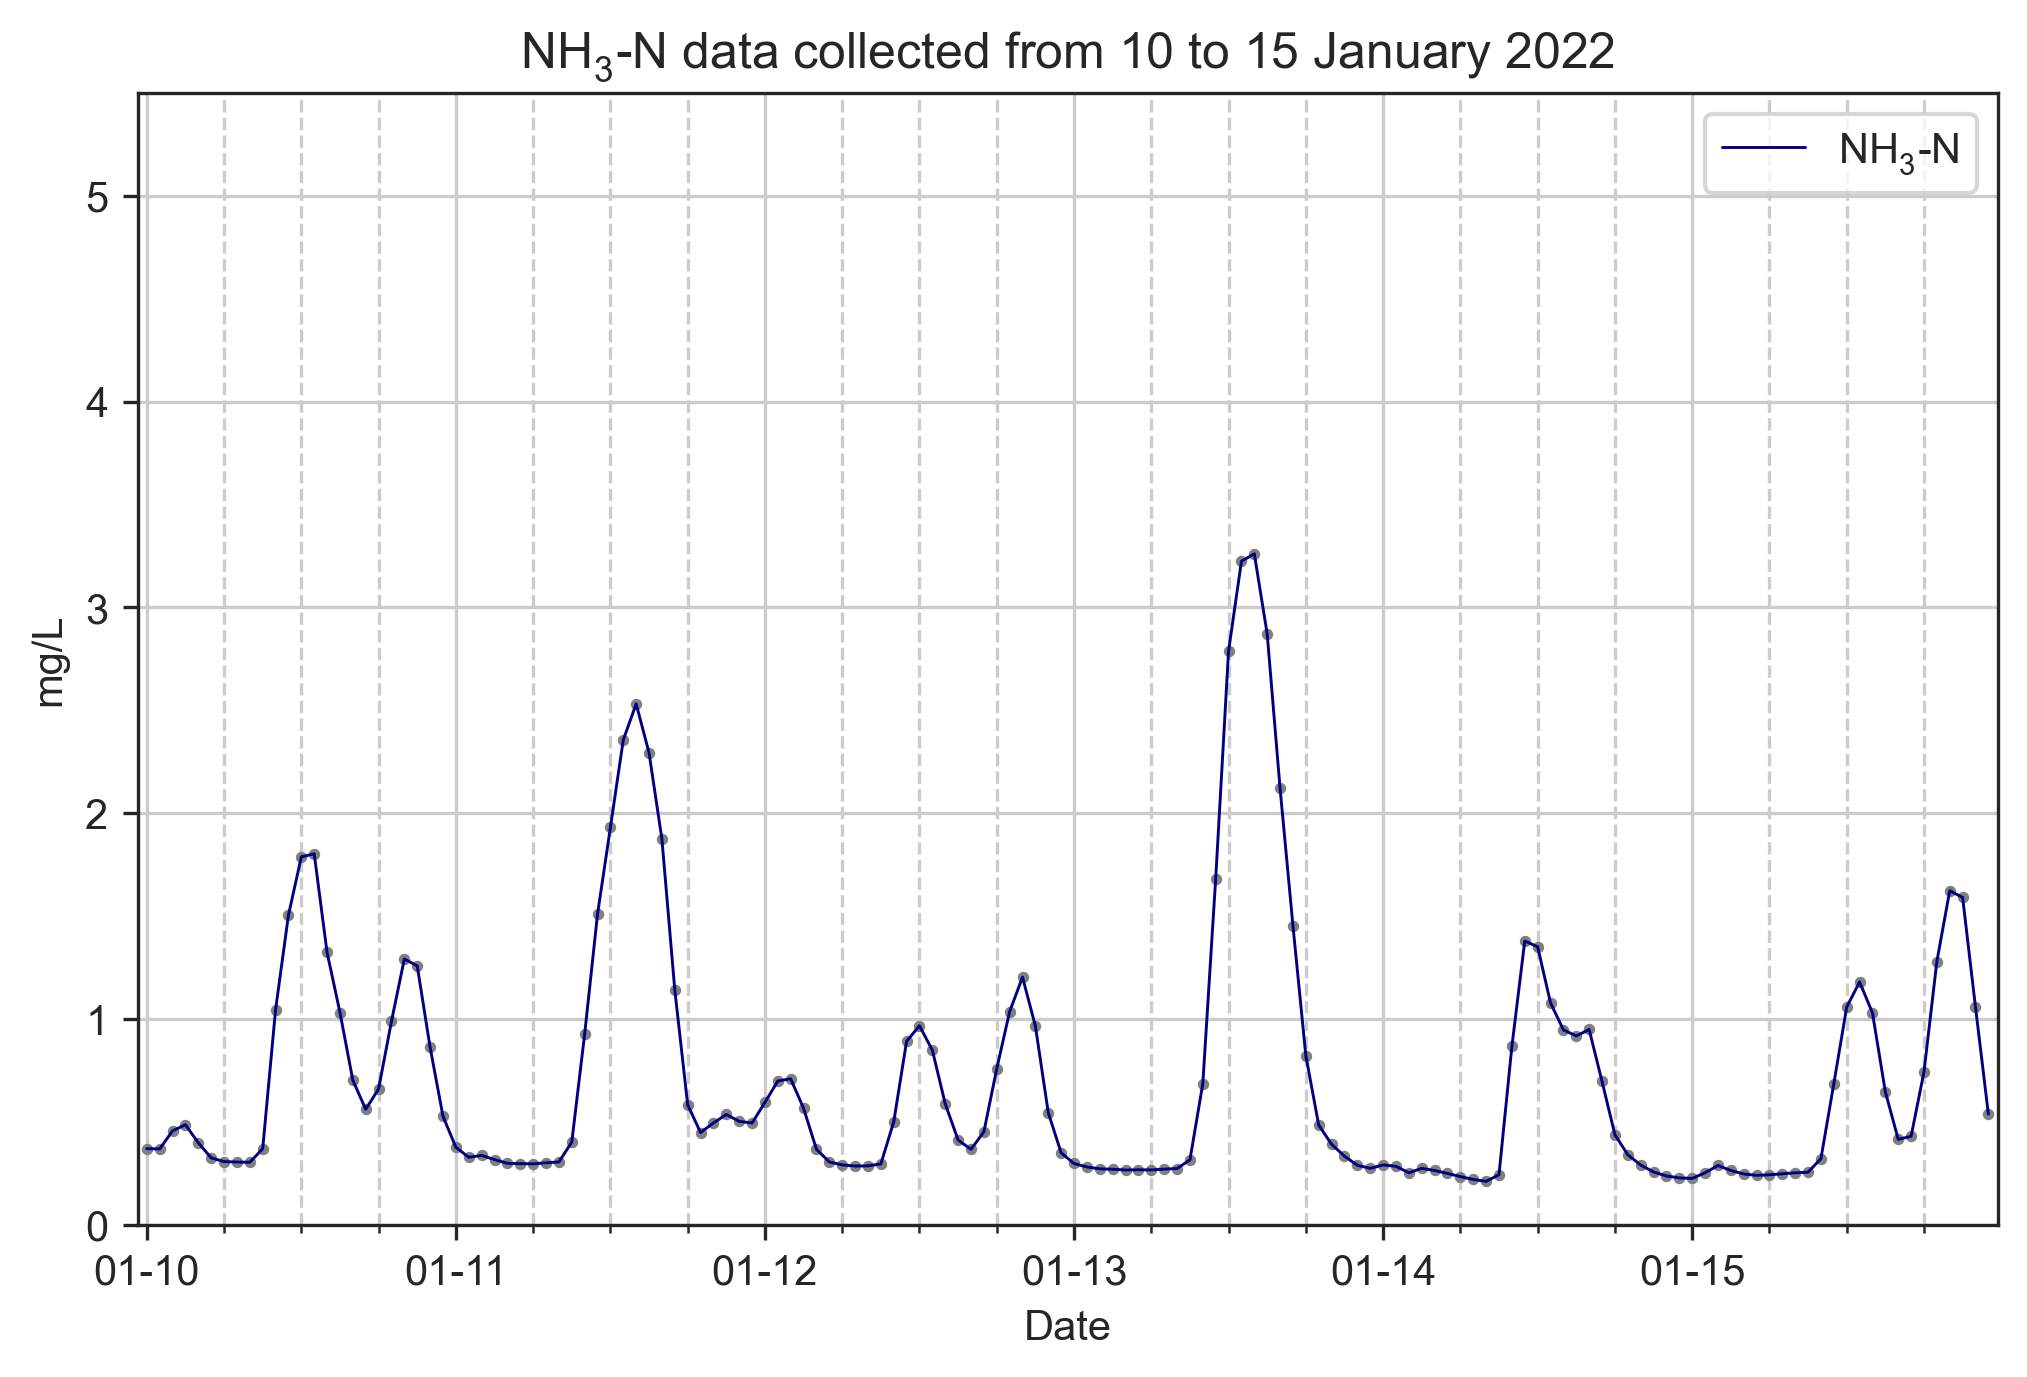
\includegraphics[width=\linewidth]{imgs/results/heterogeneity-validation.png}
    \caption{Validation dataset from January 2022.} \label{fig:valid-data}
  \end{subfigure}\\
  \begin{subfigure}[t]{0.6\textwidth}
    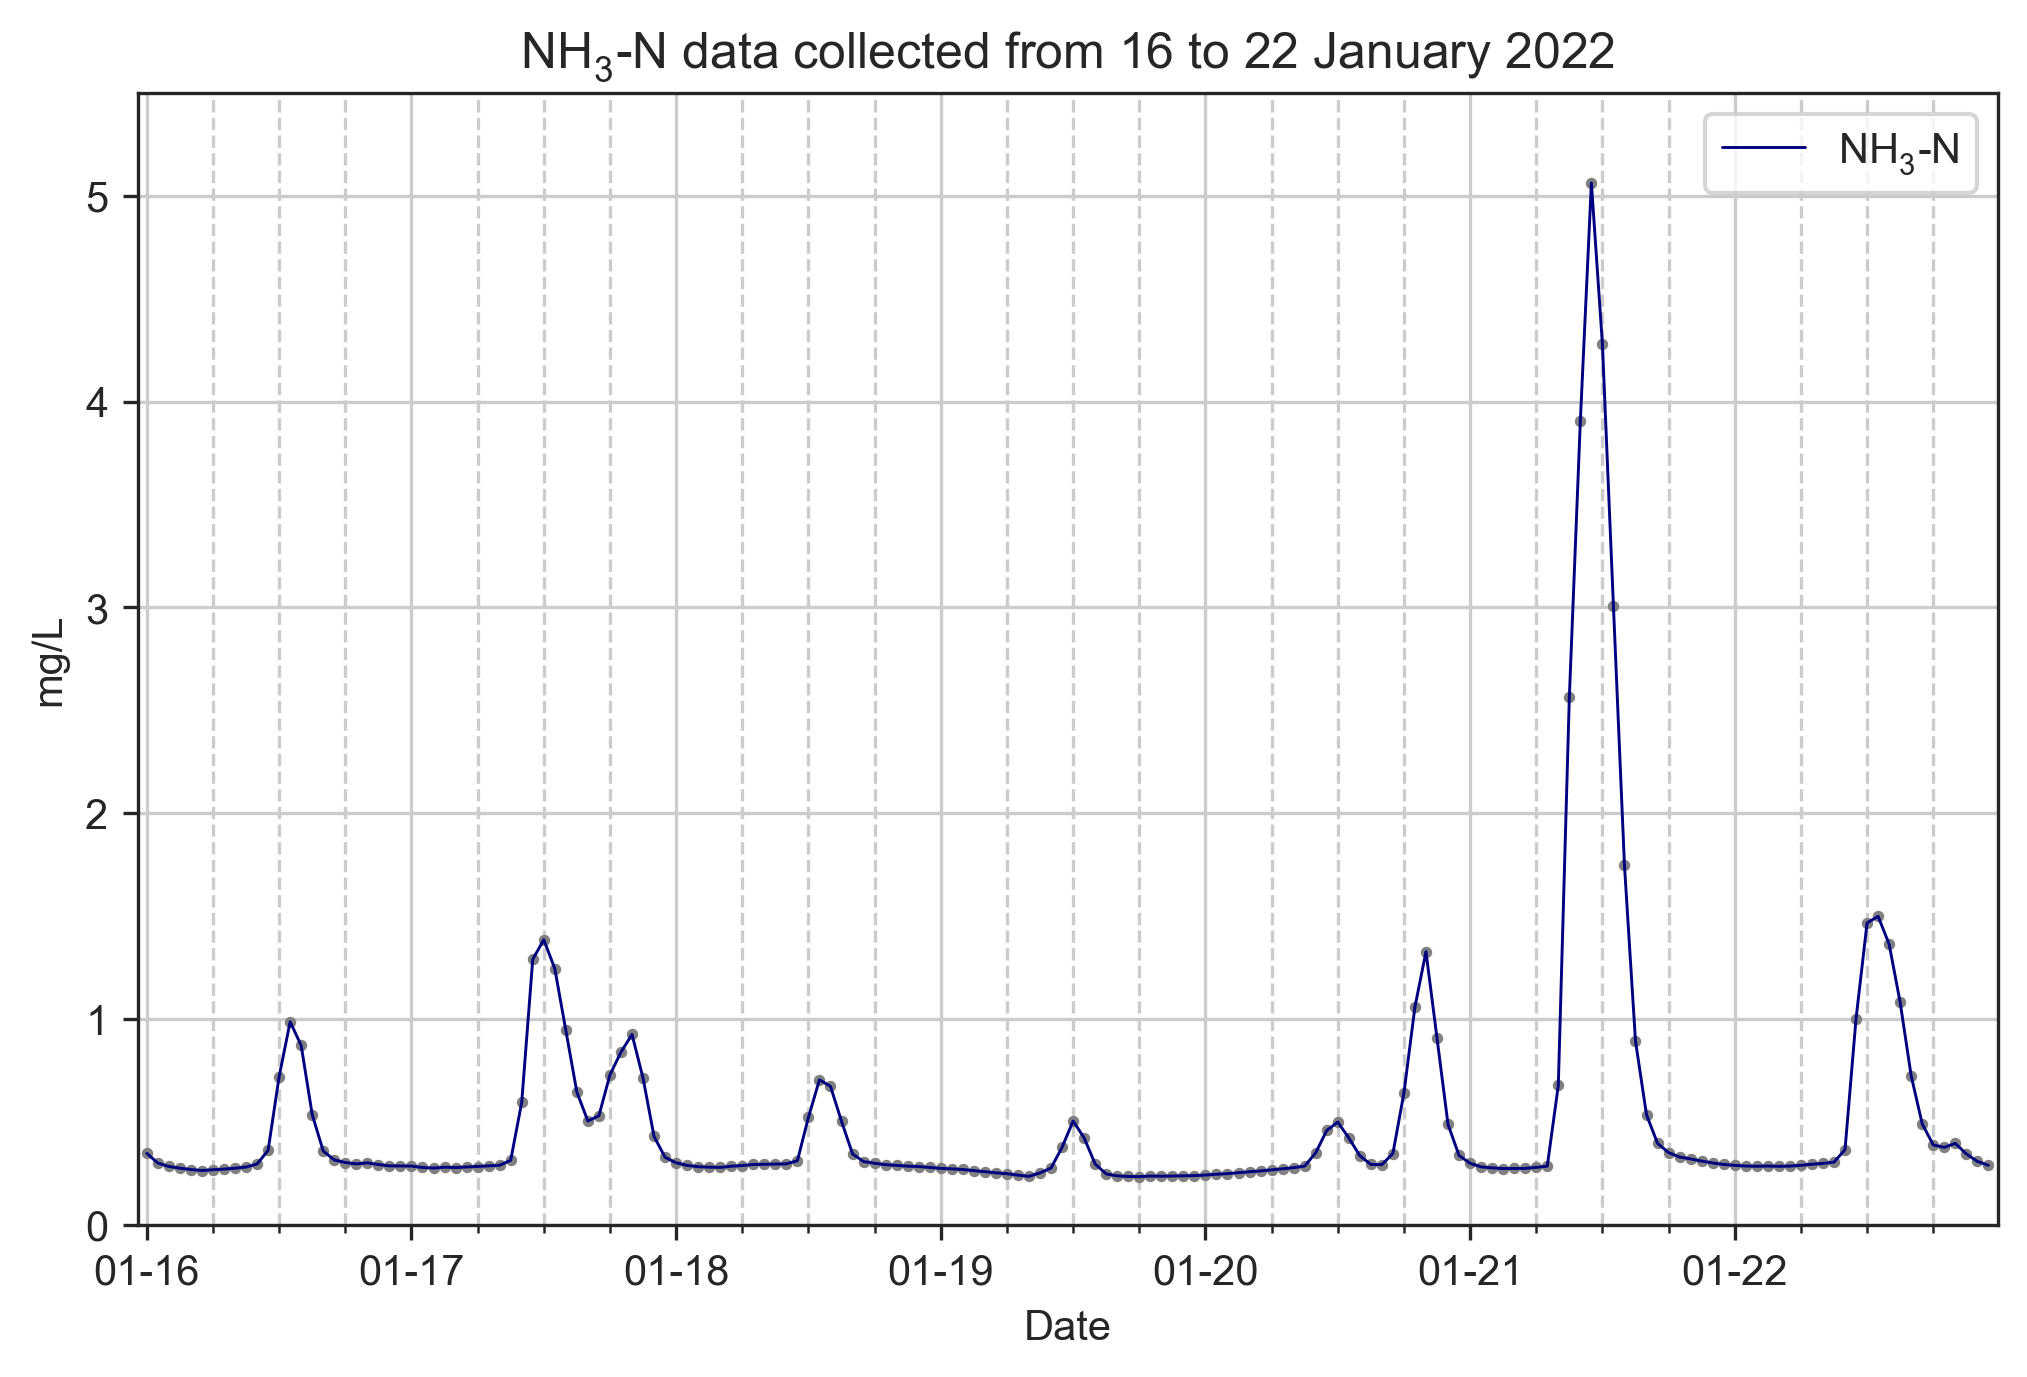
\includegraphics[width=\linewidth]{imgs/results/heterogeneity-jan-test.png}
    \caption{Testing dataset from January 2022.} \label{fig:jan-test-data}
  \end{subfigure}\\
  \begin{subfigure}[t]{0.6\textwidth}
    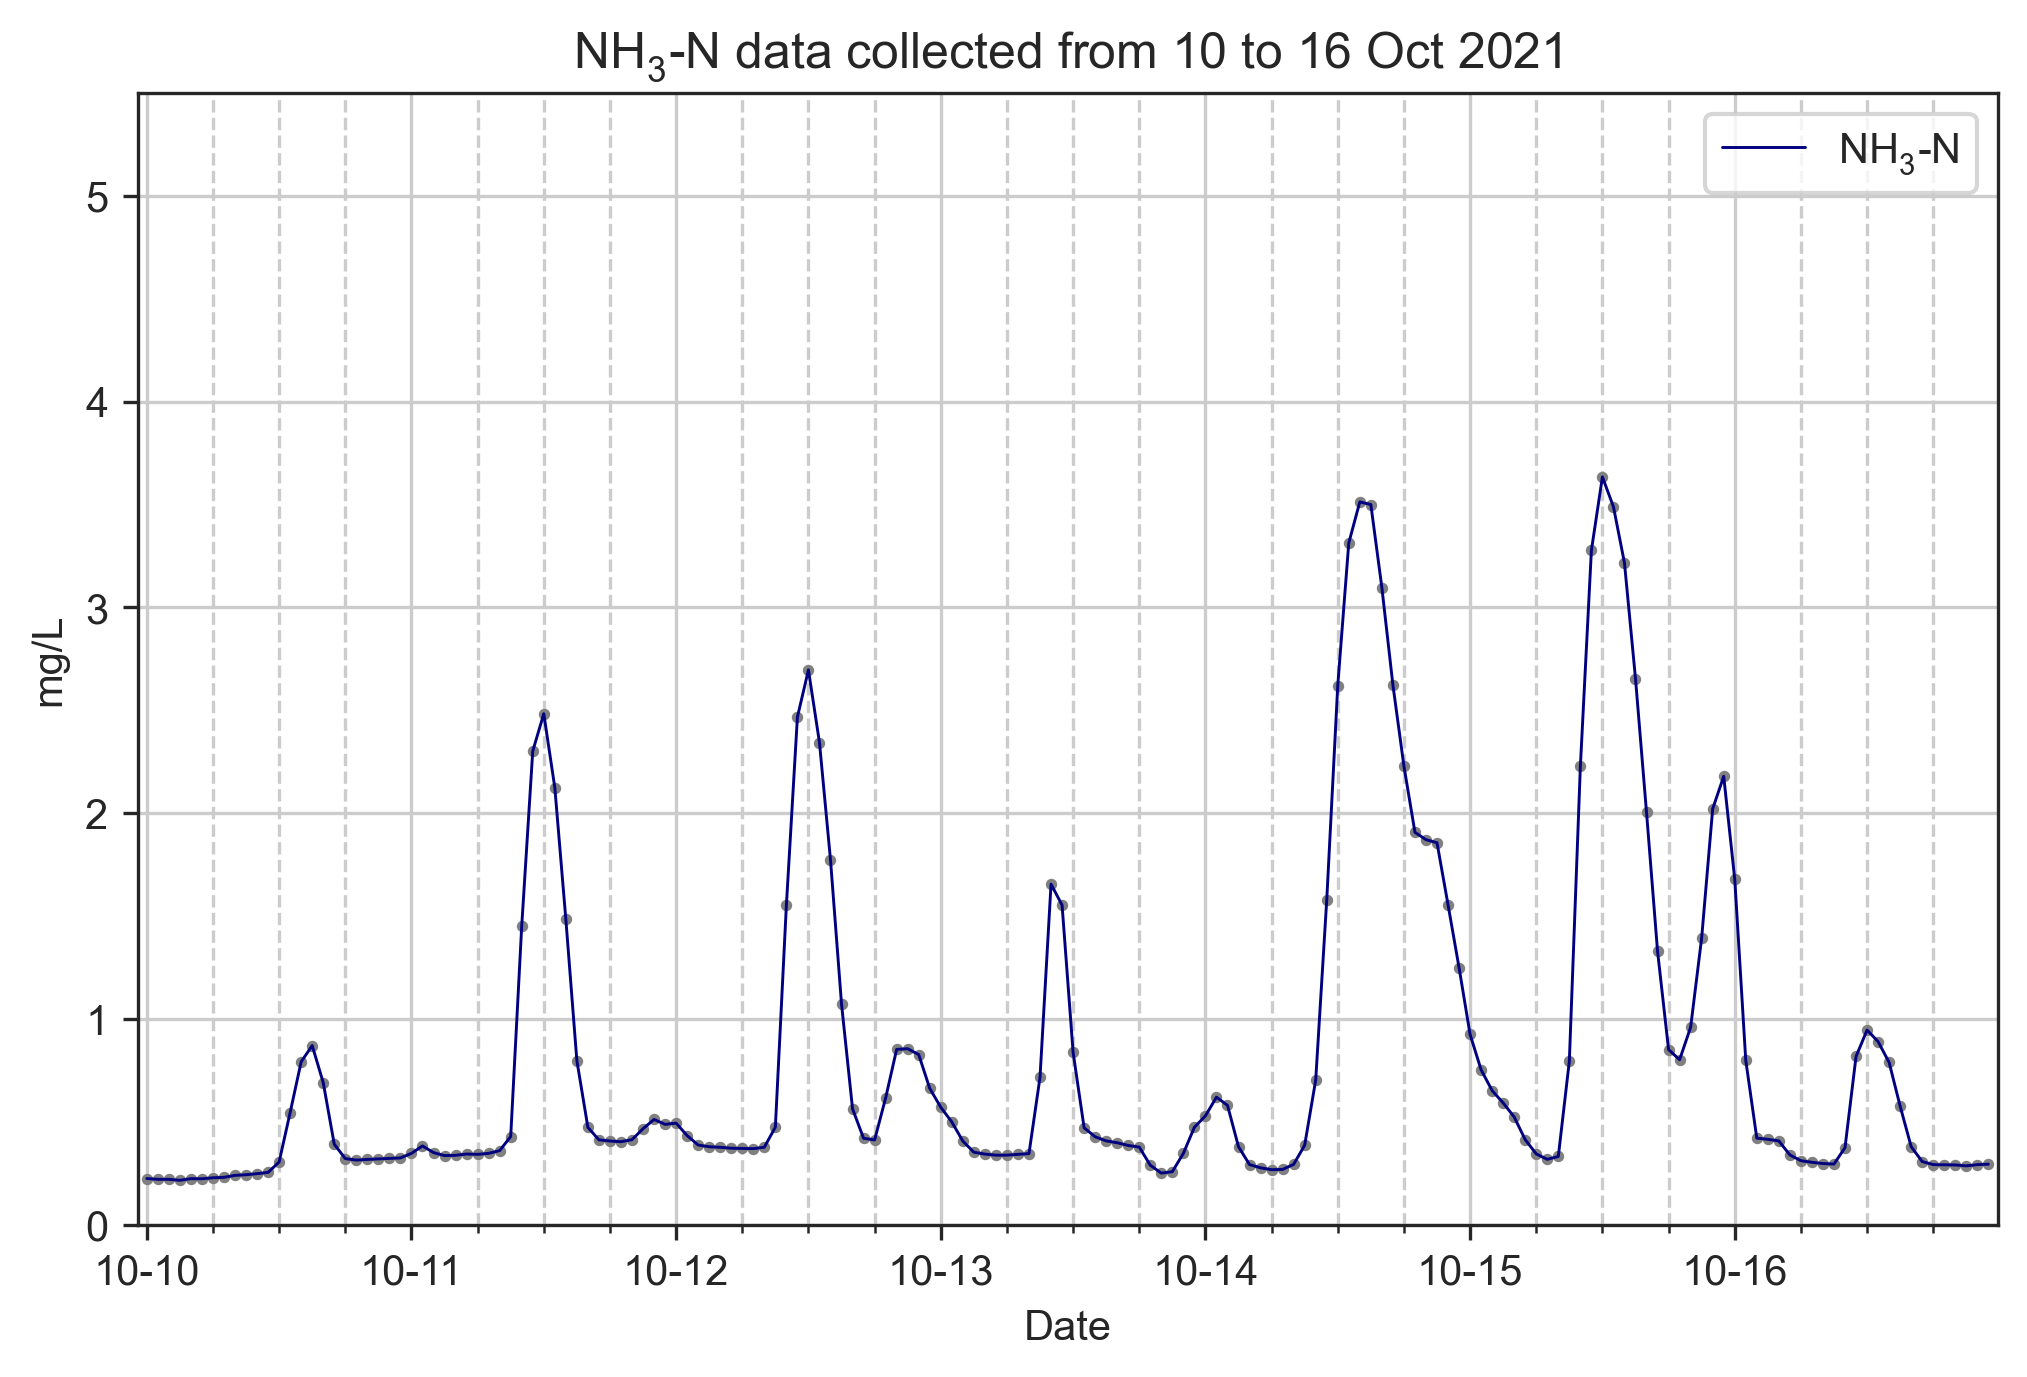
\includegraphics[width=\linewidth]{imgs/results/heterogeneity-test-oct.png}
    \caption{Testing dataset from October 2021.} \label{fig:oct-test-data}
  \end{subfigure} 
\caption{Illustration of the heterogeneity and homogeneity between validation and different testing datasets.} \label{fig:heterogeneity}
\end{figure}

%%%%%%%%%%%%%%%%%%%%%%%%%%%%%%%%%%%%%%%%%%%%%%

As shown in Table.~\ref{tab:baseline-result-oct-nh3}, the models with the top lowest test loss values are 0.0158, 0.0161, 0.0163 for LSTM-ew3, LSTM-ew2, and LSTM-ew4, which match the top three lowest validation loss values of 1.0796, 1.0969, and 0.1219. This is in good agreement with how the heterogeneity of the datasets can impact the model performance. The evaluations of the ammonia forecasting models in October 2021 showed completely different outcomes compared to those in January 2022. Instead of GRU, LSTM becomes the best model for training the ammonia forecasting model. For LSTM models, the top three Model-Dataset combinations are LSTM-ew3, LSTM-ew2, and LSTM-ew4; for GRU models, they are GRU-ew3, GRU-ew4, and GRU-ew2; for RNN models are RNN-ew4, RNN-ew2, and RNN-ew3. It is evident that EWMA filters have a more significant influence on the model performance for all the recurrent neural network models than SG filters. However, given the small dataset size, caution must be taken if the EWMA filter is applied in future works.

\begin{table}[!ht]
    \centering
    \caption{Baseline performance of ammonia forecasting model, evaluated on test dataset from \textbf{10 to 16 October 2021}. Loss values are calculated by MSE.}\label{tab:baseline-result-oct-nh3}
    \begin{NiceTabular}{lcclcc}
        \toprule
        Model-Dataset & Test loss & Valid loss & Model-Dataset & Test loss & Valid loss \\
        \midrule
        LSTM-ew3 & 0.0158 & 1.0796 & RNN-or  & 0.0197 & 1.6345 \\
        LSTM-ew2 & 0.0161 & 1.0969 & RNN-sg7 & 0.0201 & 1.6267 \\
        LSTM-ew4 & 0.0163 & 1.1219 & RNN-sg9 & 0.0205 & 1.7046 \\
        LSTM-sg5 & 0.0166 & 1.2346 & RNN-obs & 0.0206 & 1.6734 \\
        GRU-ew3  & 0.0167 & 1.2199 & DNN-ew3 & 0.0316 & 3.2317 \\
        GRU-ew4  & 0.0169 & 1.2390 & DNN-or  & 0.0316 & 3.1972 \\
        GRU-ew2  & 0.0170 & 1.1891 & DNN-sg7 & 0.0316 & 3.2014 \\
        GRU-sg9  & 0.0174 & 1.3097 & DNN-ew2 & 0.0318 & 3.1677 \\
        LSTM-obs & 0.0175 & 1.2366 & DNN-ew4 & 0.0319 & 3.2188 \\
        LSTM-or  & 0.0177 & 1.2612 & DNN-obs & 0.0319 & 3.2383 \\
        GRU-sg5  & 0.0178 & 1.2644 & DNN-sg5 & 0.0319 & 3.2170 \\
        GRU-sg7  & 0.0180 & 1.2508 & DNN-sg9 & 0.0319 & 3.2484 \\
        LSTM-sg7 & 0.0180 & 1.1804 & RF-sg9  & 0.1307 & - \\
        GRU-or   & 0.0187 & 1.3993 & RF-sg7  & 0.1311 & - \\
        LSTM-sg9 & 0.0188 & 1.3076 & RF-sg5  & 0.1343 & - \\
        GRU-obs  & 0.0189 & 1.3638 & RF-ew2  & 0.1346 & - \\
        RNN-ew4  & 0.0190 & 1.5992 & RF-ew3  & 0.1368 & - \\
        RNN-ew2  & 0.0191 & 1.5425 & RF-obs  & 0.1443 & - \\
        RNN-ew3  & 0.0193 & 1.6041 & RF-ew4  & 0.1451 & - \\
        RNN-sg5  & 0.0195 & 1.5088 & RF-or   & 0.1477 & - \\
        \bottomrule
    \end{NiceTabular}
\end{table}

The test loss values of the colour forecasting models are presented in Table.~\ref{tab:baseline-result-jan-colour}. The top six lowest test loss models are LSTM-ew4, LSTM-ew2, LSTM-ew3, GRU-ew3, GRU-ew2, and GRU ew4 with the values of 0.0136, 0.0138, 0.0138, 0.0140, 0.0142, and 0.0143, respectively. LSTM models are shown to be the best-performanced model in forecasting colour levels. The results also suggest that all the top lowest test loss models are trained by EWMA filtered datasets. We found that LSTM, GRU, and RNN models trained by EWMA filtered datasets generated the top lowest test loss values compared to the same models trained by SG filtered datasets. Interestingly, in both colour and ammonia forecasting models, LSTM models trained by EWMA filtered dataset showed the most superior performance, as shown in Table.~\ref{tab:baseline-result-oct-nh3} and Table.~\ref{tab:baseline-result-jan-colour}. LSTM models trained with EWMA filtered datasets are proved to be the best model and pre-processing techniques for training colour forecasting models in this study.

In the investigation of how a small dataset can influence the model results, we found that the top three lowest validation loss values are LSTM-sg9, LSTM-sg7, and LSTM-ew4, which rank the $7^{th}$, $20^{th}$, and $1^{st}$ as the lowest test loss values. In this study, there is no extra colour testing dataset we can retrieve from the historical dataset, despite the fact that we were keen to investigate the homogeneity and heterogeneity of the colour validation and testing dataset. Compromises have to be made during the analysis of colour forecasting models.

\begin{table}[!ht]
  \centering
  \caption{Baseline performance of colour forecasting model, evaluated on test dataset from \textbf{16 to 22 Janurary 2022}. Loss values are calculated by MSE.}\label{tab:baseline-result-jan-colour}
  \begin{NiceTabular}{lcclcc}
      \toprule
      Model-Dataset & Test loss & Valid loss & Model-Dataset & Test loss & Valid loss \\
      \midrule
      LSTM-ew4 & 0.0136 &0.7515&RNN-obs  & 0.0160 &1.0623 \\
      LSTM-ew2 & 0.0138 &0.8011&LSTM-sg7 & 0.0161 &0.7439 \\
      LSTM-ew3 & 0.0138 &0.7547&LSTM-sg5 & 0.0168 &0.8355 \\
      GRU-ew3  & 0.0140 &0.8068&DNN-sg5  & 0.0180 &1.4702 \\
      GRU-ew2  & 0.0142 &0.8330&DNN-sg7  & 0.0180 &1.4823 \\
      GRU-ew4  & 0.0143 &0.7694&DNN-sg9  & 0.0180 &1.4574 \\
      LSTM-sg9 & 0.0143 &0.7137&DNN-ew4  & 0.0181 &1.4632 \\
      RNN-ew3  & 0.0144 &0.8492&DNN-ew3  & 0.0182 &1.4716 \\
      RNN-ew4  & 0.0147 &0.8476&DNN-ew2  & 0.0183 &1.4946 \\
      RNN-sg9  & 0.0147 &0.8363&DNN-obs  & 0.0186 &1.5397 \\
      LSTM-obs & 0.0148 &0.9744&RF-sg9   & 63.6847& \\
      GRU-obs  & 0.0149 &0.9927&RF-sg7   & 73.8263& \\
      RNN-ew2  & 0.0150 &0.9083&RF-ew3   & 75.1974&- \\
      GRU-sg9  & 0.0151 &0.7575&RF-ew4   & 77.8829&- \\
      RNN-sg5  & 0.0158 &0.8846&RF-obs   & 78.5296&- \\
      RNN-sg7  & 0.0158 &0.8755&RF-ew2   & 78.8753&- \\
      GRU-sg7  & 0.0159 &0.7791&RF-sg5   & 81.0696&- \\
      GRU-sg5  & 0.0160 &0.8080&    -    &     -  &- \\
      \bottomrule
  \end{NiceTabular}
\end{table}

By comparing the baseline performance and the influences of data pre-processing techniques on machine learning models, our findings appear to be well substantiated by using LSTM models for training ammonia and colour forecasting models due to their outstanding model performance evaluated by test loss values. Although EWMA filters showed surprising effects on improving the performance of most models, the conclusions of determining which pre-processing techniques are the optimum option should be treated with caution. Thus, the testings of the proposed model training processes will include all the pre-processing techniques for model training, and LSTM will be used as the only machine learning model.

\subsection{The effect of window size of data smoothing filters}

\begin{figure}[!ht]
  \centering
  \begin{subfigure}[t]{0.75\textwidth}
    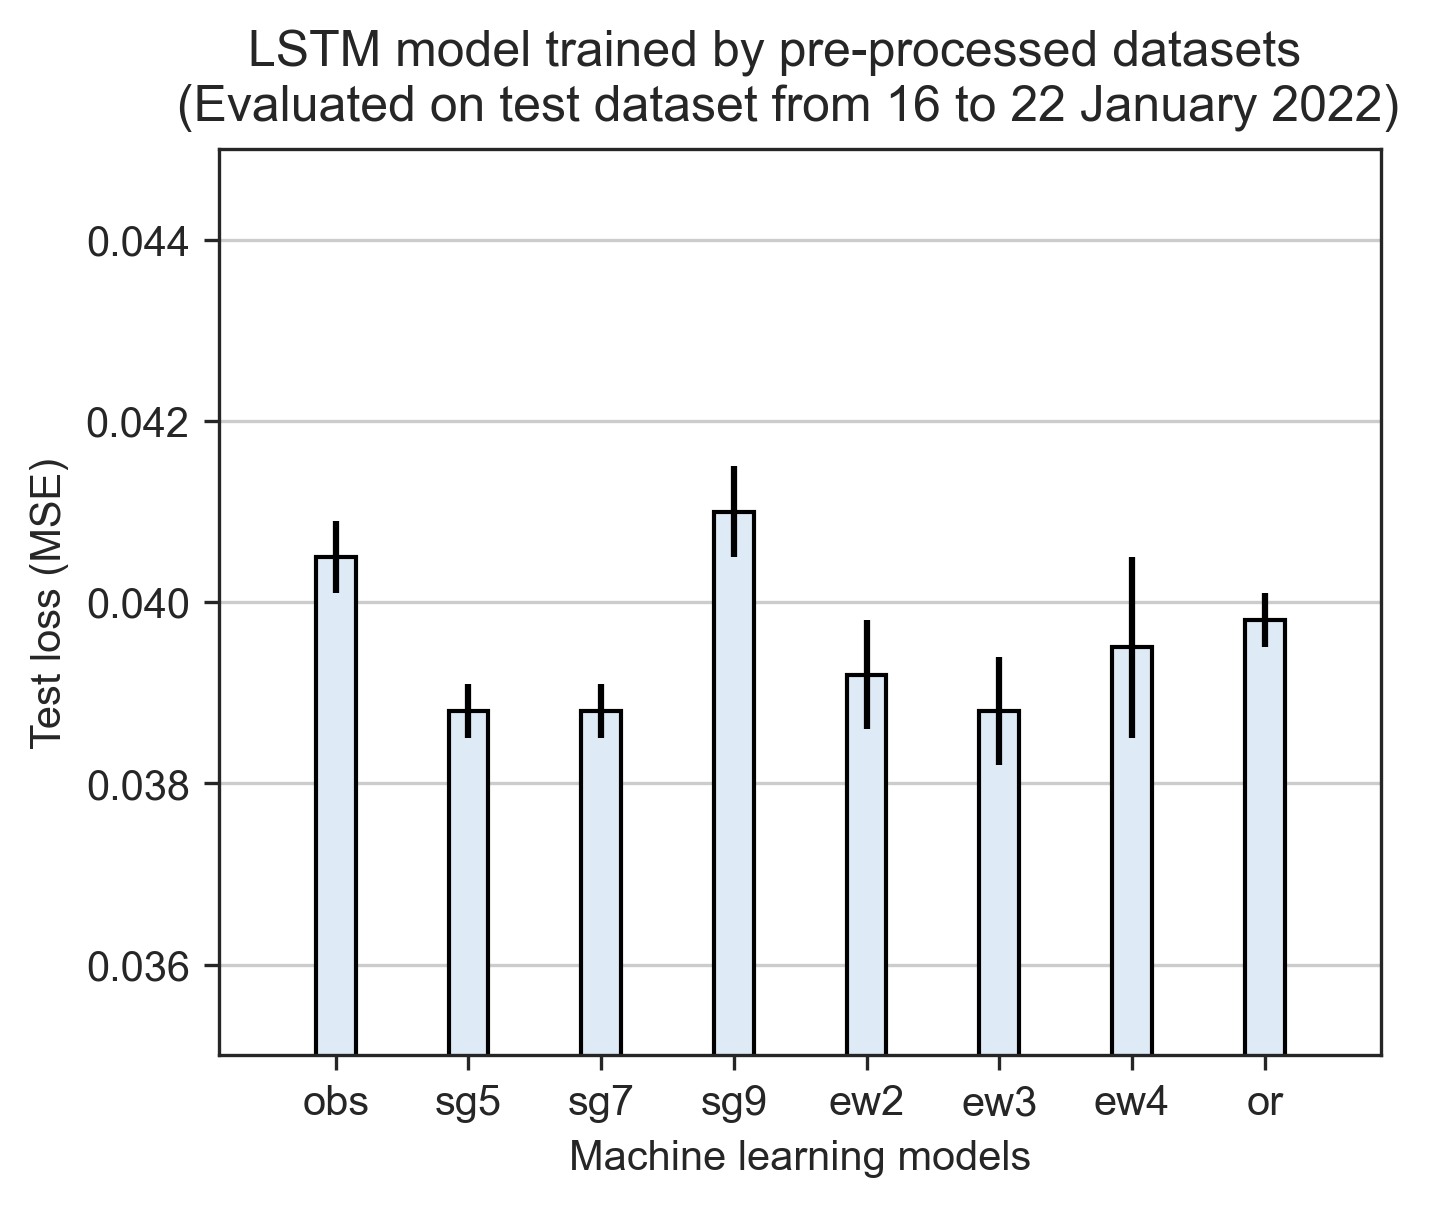
\includegraphics[width=\linewidth]{imgs/results/feature-engineering/pre-processing-nh3-jan.png}
    \caption{Baseline performance of ammonia forecasting models trained by LSTM.} \label{fig:preprocessing-nh3}
  \end{subfigure}
  \hspace{2em}
  \begin{subfigure}[t]{0.75\textwidth}
    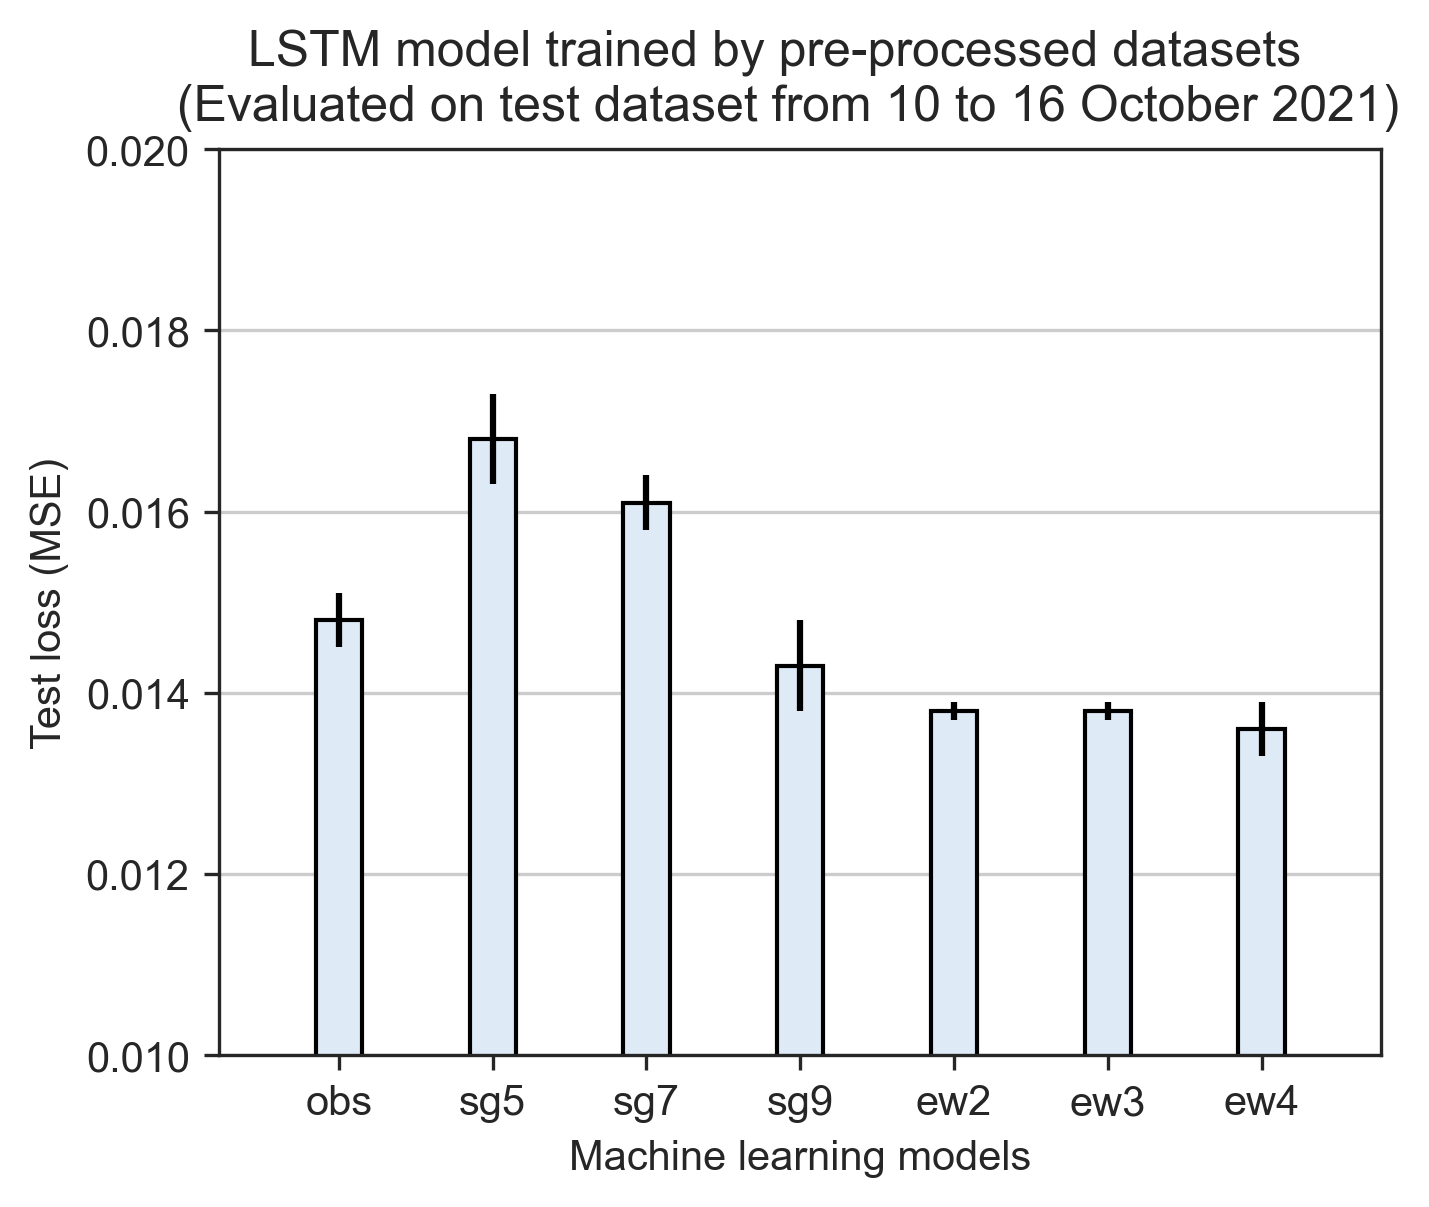
\includegraphics[width=\linewidth]{imgs/results/feature-engineering/pre-processing-colour.png}
    \caption{Baseline performance of colour forecasting models trained by LSTM.} \label{fig:preprocessing-colour}
  \end{subfigure}
\caption{Baseline performance of ammonia and colour forecasting models.} \label{fig:preprocessing-comparison}
\end{figure}

The influences of window sizes in the data smoothing process are investigated using LSTM models and illustrated in Fig.~\ref{fig:preprocessing-comparison}. Larger and smaller SG window sizes have different impacts on ammonia and colour forecasting models. In ammonia forecasting models, as shown in Fig.~\ref{fig:preprocessing-nh3}, LSTM models trained with SG filtered datasets with window sizes of 5, 7, and 9 have the test loss values of 0.0388, 0.0388, and 0.0410. The results suggested that modifying data points at higher degrees may negatively affect the model training process. The results from models trained by EWMA filtered datasets showed good agreement with this finding. The model trained with EWMA filtered datasets with the windows size of 2, 3, and 4 have the test loss values of 0.0392, 0.0388, and 0.0395. A higher test loss value is observed in LSTM-ew4 compared to LSTM-ew3.

For colour forecasting models, as shown in Fig.~\ref{fig:preprocessing-colour}, LSTM models trained by SG filtered datasets with window sizes of 5, 7, and 9 have test loss values of 0.0168, 0.0161, and 0.0143. LSTM models trained by EWMA filtered datasets with window sizes of 2, 3, and 4 showed test loss values of 0.0138, 0.0138, and 0.0136. From these results, we observed that larger window sizes helped the models achieve lower test loss for colour forecasting models, which does not support what we have concluded for the ammonia forecasting models. One possible explanation for the contradictory results is that ammonia and colour data have different sensitivity toward the data smoothing filters. For instance, ammonia concentrations change between the values of 1.0 to 7.0 mg/L, while colour levels vary from 80 to 160 Hazen Units, making the values of filtered data points less significant in colour data. In other words, if ammonia data points are shifted from the original values after applying data smoothing techniques, the values might be biased considering the fluctuated range of ammonia is small, while the shifted colour level data can be less biased among the sample regarding the fluctuation range of colour level is much larger. By far, we can not conclude how to select the window sizes of the data smoothing filters. The unpredictable influences of applying data smoothing filters on forecasting models impede the determination of the optimum data smoothing techniques in the subsequent experiments. 

\section{Exploit hidden patterns in MBR effluent water quality to enhance model performance}
\subsection{Ammonia forecasting models}
In the section of feature engineering, we have introduced the selection and creation of the extra input features for training forecasting models, as shown in Fig.~\ref{fig:feature-selection}. In this study, a forecasting model trained by one feature is called an univariate model and denoted as LSTM-1; a forecasting model trained by two features is called a multivariate model and denoted as LSTM-2. For models trained by three and four features are denoted as LSTM-3 and LSTM-4. In Fig.~\ref{fig:nh3-feature-engineering}, the performance of ammonia forecasting models trained by two to four inputs (i.e., LSTM-2, LSTM-3, LSTM-4) is compared with the baseline performance (i.e., LSTM-1-obs) to demonstrate how the feature engineered features influenced on the model outputs. 
%Notice that due to colour data are not available from 10 to 16 October 2021, the models in Fig.~\ref{fig:colour-feature-engineering} were evaluated on training dataset from 16 to 22 January 2022. 

As shown in Fig.~\ref{fig:nh3-feature-engineering}, LSTM-4-obs, LSTM-3-obs, LSTM-2-obs, and LSTM-1-obs have the test loss values of 0.0432, 0.0426, 0.0411, and 0.0405, respectively. This result indicates that LSTM models trained with more features resulted in poorer model performance. Based on our understanding to the extra features such as color levels and sine/cosine features, models trained with more features are expected lower test values. The model performance from LSTM-sg7 and LSTM-sg9 fits well with what we hypothesized. The test loss values of LSTM-4-sg7, LSTM-3-sg7, LSTM-2-sg7, LSTM-1-sg7 are 0.0369, 0.0373, 0.0379, 0.0388, respectively. For LSTM-4-sg9, LSTM-3-sg9, LSTM-2-sg9, and LSTM-1-sg9, the test loss values are 0.0384, 0.0391, 0.0409, 0.0410, respectively. These findings showed that the test loss values of the LSTM models trained by sg7 and sg9 filtered datasets followed the trends of LSTM-4 $<$ LSTM-3 $<$ LSTM-2 $<$ LSTM-1. The most remarkable results are from LSTM models trained by SG filtered dataset at a window size of 7. Comparing to the baseline model performance (i.e., LSTM-1-obs), the test loss values of LSTM-1-sg7, LSTM-2-sg7, LSTM-3-sg7 and LSTM-4-sg7 reduced by 4.2\%, 6.4\%, 7.9\%, and 8.9\%, respectively.

Our findings in the ammonia forecasting models suggest that colour level is an indispensable feature for improving the model performance. LSTM-2 models trained by datasets applied with any pre-processing techniques showed lower test loss compared to LSTM-1, except LSTM-2 trained by dataset without applying any methods. Strong evidence leads us to believe that the fluctuation of ammonia concentration is highly correlated with the colour levels in SHWEPP influent even without direct evidence.

The methods of training LSTM models on pre-processed datasets have proved their benefits in improving baseline model performance. Yet, the test loss values were only reduced slightly for those models trained with EWMA filtered datasets. As shown in Fig.~\ref{fig:nh3-feature-engineering}, LSTM-3-ew2, LSTM-4-ew2, LSTM-3-ew4, and LSTM-4-ew4 shared very similar test loss values to LSTM-1-obs, indicating the advantages of enhanced training datasets were not fully reflected on the model performance when LSTM models were trained with EWMA filtered datasets.

\begin{figure}[!ht]
    \centering
    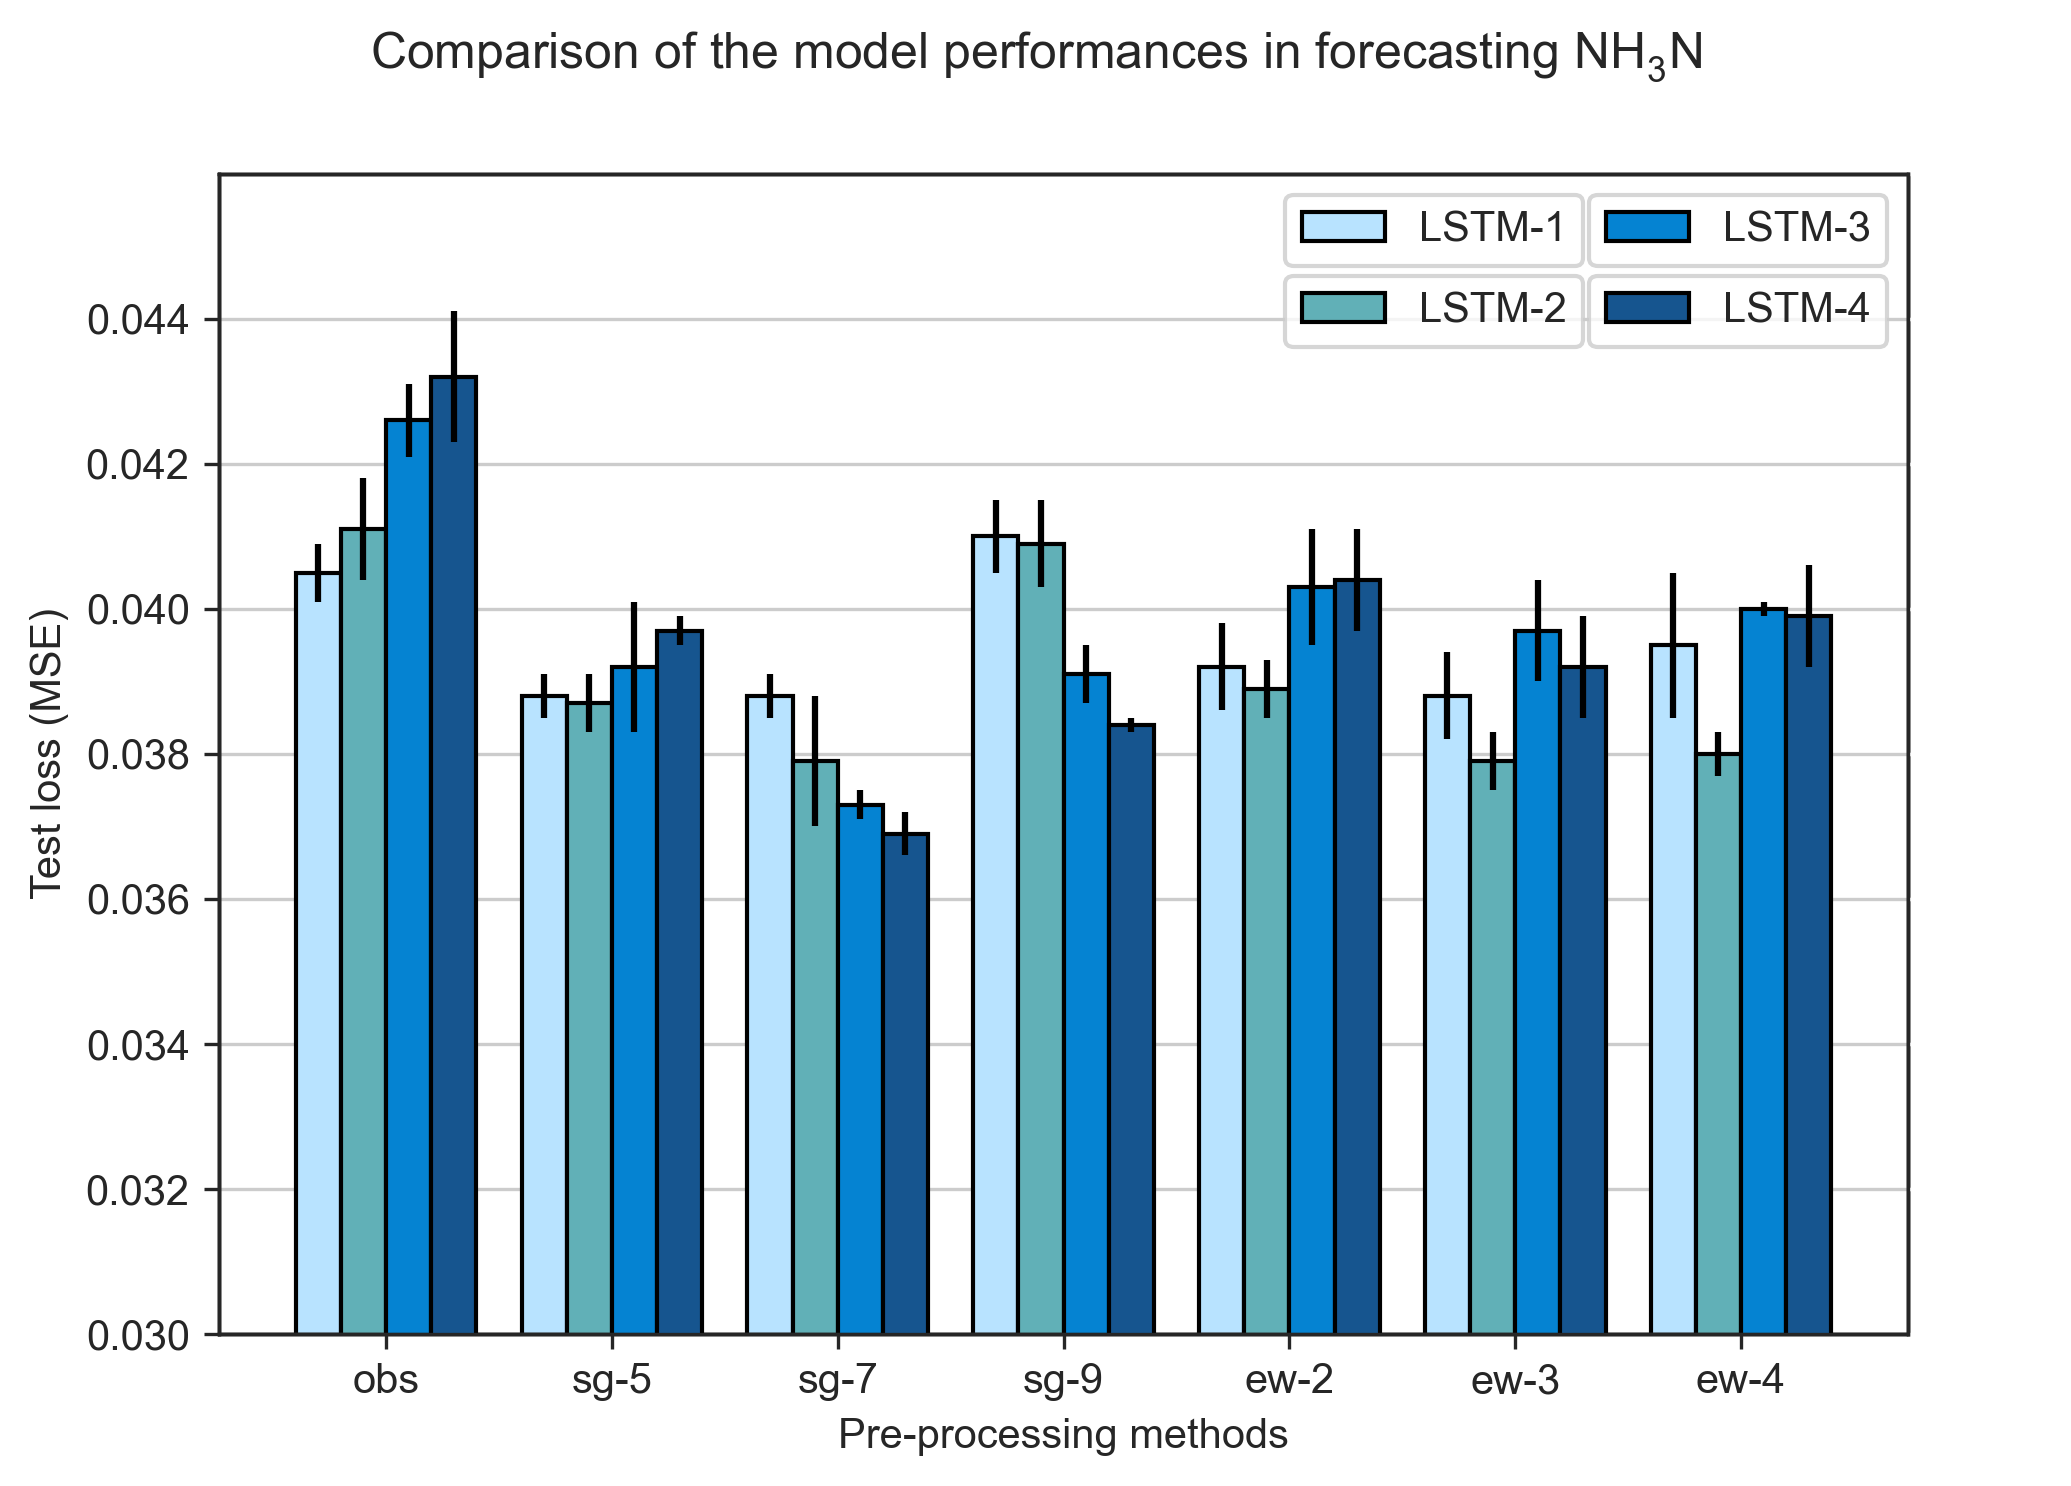
\includegraphics[width=1.0\columnwidth]{imgs/results/feature-engineering/nh3-input-1-4-comparison.png}
    \caption{Comparisons of the model performance in forecasitng ammonia concentrations.}
    \label{fig:nh3-feature-engineering}
 \end{figure}

\subsection{Colour forecasting models}

As shown in Fig.~\ref{fig:colour-feature-engineering}, the baseline performance is LSTM-1-obs with test loss value of 0.0148, and many models trained by both SG and EWMA filtered datasets show lower test loss values. The performance of models trained by SG filtered datasets was rather disappointing. In the results of models trained by sg-5 and sg7 filtered datasets, only LSTM-3-sg5, LSTM-3-sg7, and LSTM-4 sg-7 showed lower test loss values of 0.0144, 0.0143, and 0.0136, respectively, compared to LSTM-1-obs. Models trained by sg9 and all the EWMA filtered datasets showed improvement over LSTM-1-obs. In LSTm-3-sg9, we observed the lowest test loss value of 0.0129, which is 28.6\% lower than the test loss values of 0.0148 from LSTM-1-obs. 

The test loss values of LSTM-4-sg9, LSTM-4-ew2, LSTM-4-ew3, and LSTM-4-ew4 are higher than LSTM-3-sg9, LSTM-3-ew2, LSTM-3-ew3, and LSTM-3-ew4, by 0.0009, 0.0009, 0.0002, and 0.0002, respectively. This finding indicates that training with ammonia and the sine/cosine features deteriorate the model performance for color forecasting models. From what we found in the results of ammonia forecasting models, we concluded that the test loss values increase more when more features were input to the training datasets. In the colour forecasting results, the finding contrasts what we have found previously. 

The interpretation for the higher test loss in LSTM-4 models in sg9, ew2, ew3, and ew4 filtered datasets compared to LSTM-3 and LSTM-2 models is that ammonia and sine/cosine features are irrelevant to the development of colour forecasting models. In the process of generating feature engineering, we observed that colour substances are mixed with municipal wastewater at the volume to volume ratio of 1 to 50. Hence, we can infer that the model outputs of forecasted colour levels are highly subject to the input of ammonia concentration. In the training process of the machine learning model, the model treats each input feature with equivalent importance; however, when the model is trained and input with unseen data, the model cannot differentiate which input feature actually influences more on the model outputs. The results suggest that it is best to train features of colour data and sin/cosine features for training color forecasting models.

%\noindent
%\begin{myenumerate}
%    \item In the results of LSTM-sg7, the test values decreased with the increased number of model inputs, which satified the hypothesis we claimed in previous section.
%    \item The test loss values of LSTM-2 in all the pre-processed datasets are lower than LSTM-1 except for LSTM-obs, LSTM-sg9 and LSTM-ew2.
%    \item In LSTM-obs, models trained with more inputs resulted in poorer model performance, except for LSTM-obs, LSTM-sg9 and LSTM-ew2.
%\end{myenumerate}

\begin{figure}[!ht]
    \centering
    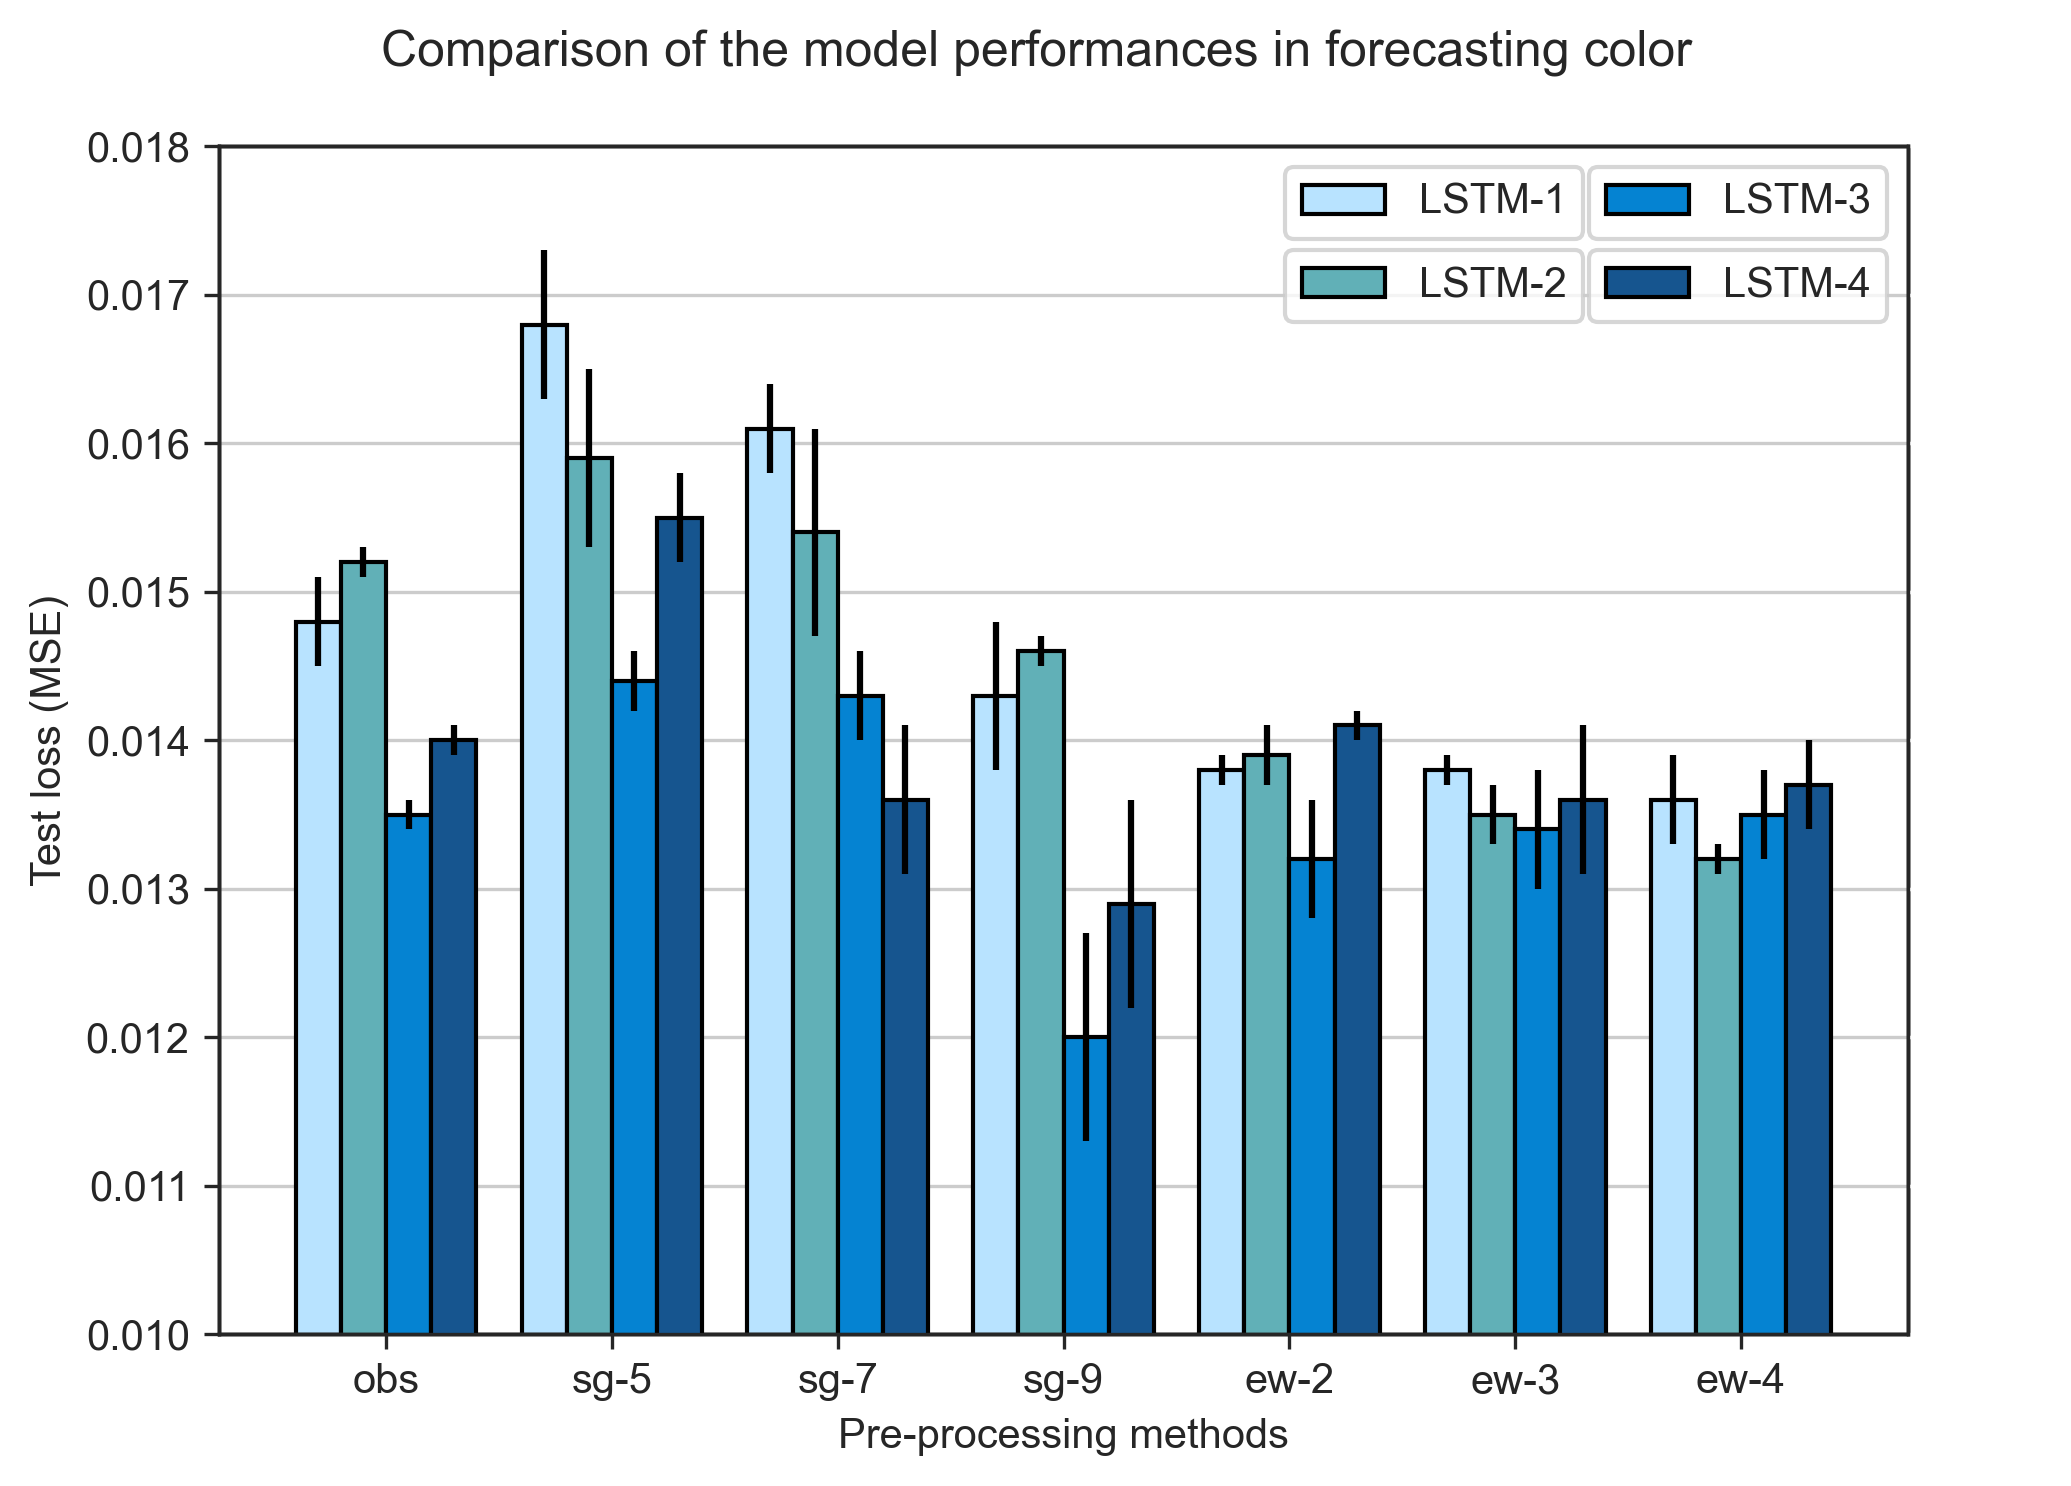
\includegraphics[width=1.0\columnwidth]{imgs/results/feature-engineering/colour-input-1-4-comparison.png}
    \caption{Comparisons of model performance in forecasting colour levels.}
    \label{fig:colour-feature-engineering}
 \end{figure}

%\section{Design of model architecture through analyzing wastewater composition in sewer system}

\subsection{Model forecasting results on different forecast horizon}
In this study, ammonia and colour forecasting models were input with data from the past 24 hours to forecast the values three hours into the future. To demonstrate how the proposed model training methods improved the baseline model performance, the forecasted results were visualized for easier comparisons. As shown in Fig.~\ref{fig:nh3-forecast-fc1}, the proposed model training methods helped the model to forecast better on 21 January as in Fig.~\ref{fig:nh3-lstm-4-fc1} during the low ammonia concentration period. On other days, both LSTM-1-obs and LSTM-4-sg7 shared similar accuracy in forecasting ammonia concentration.

\begin{figure}[!ht]
  \centering
  \begin{subfigure}[t]{0.75\textwidth}
    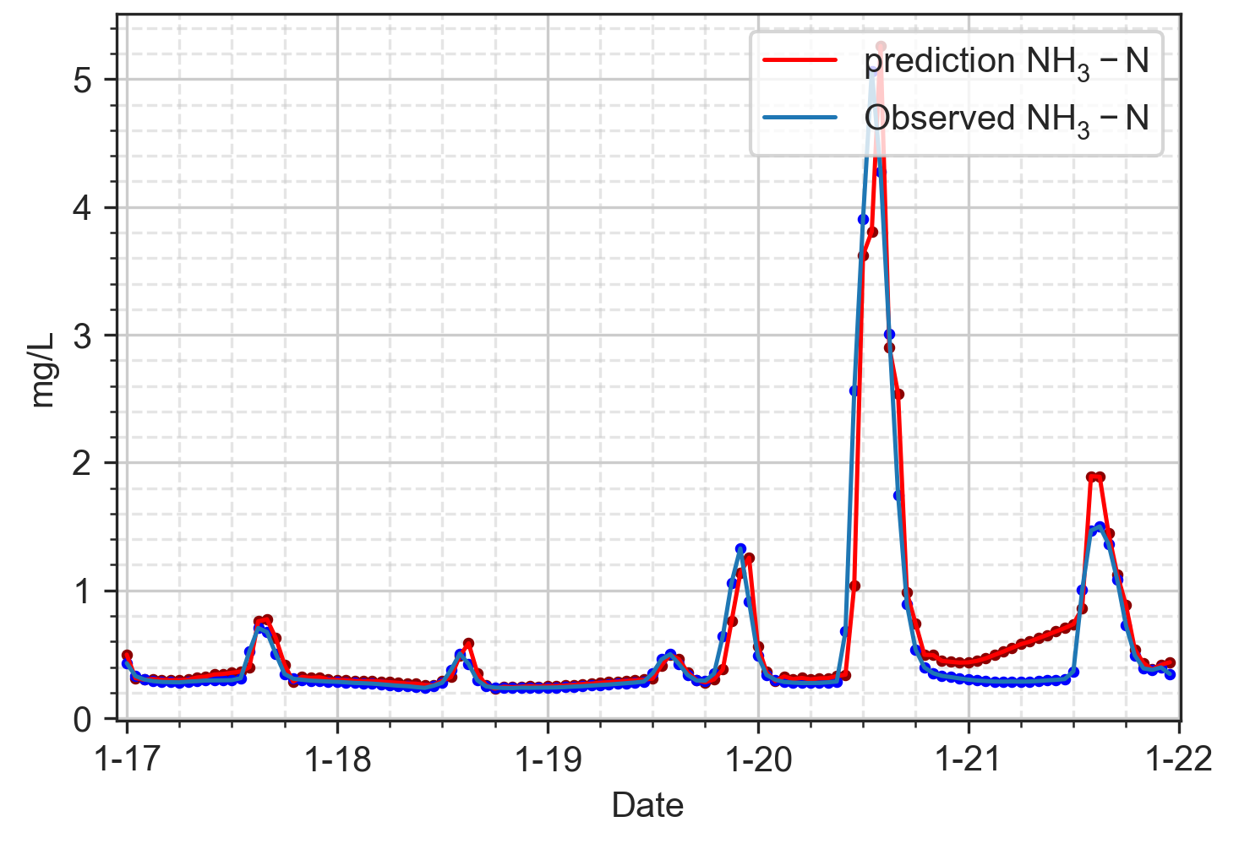
\includegraphics[width=\linewidth]{imgs/results/steps/nh3-lstm-1-fc1.png}
    \caption{LSTM-1-obs, MSE = 0.0647} \label{fig:nh3-lstm-1-fc1}
  \end{subfigure}\\
  \vspace{2em}
  \begin{subfigure}[t]{0.75\textwidth}
    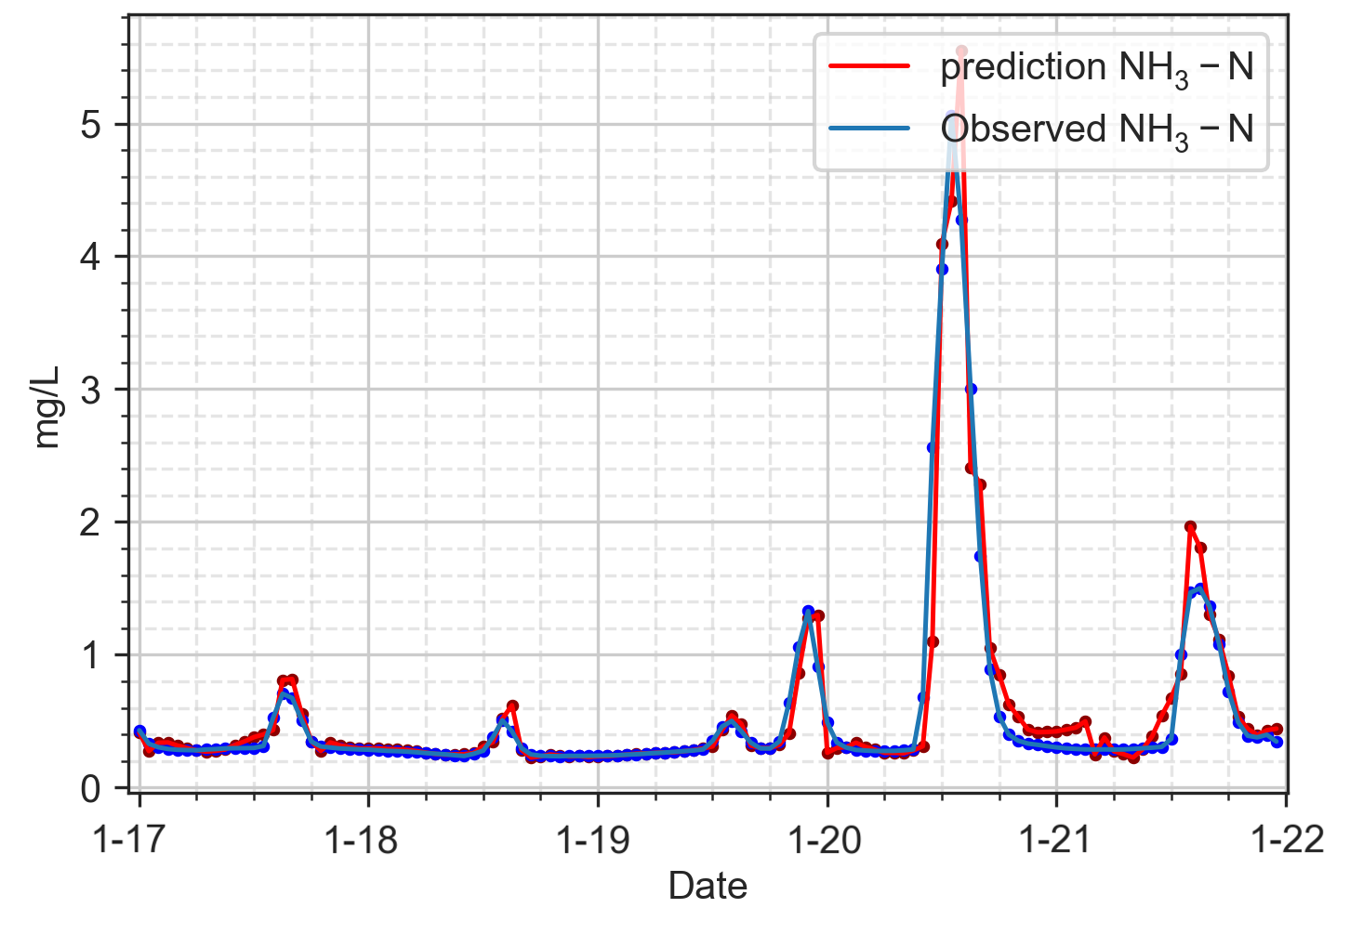
\includegraphics[width=\linewidth]{imgs/results/steps/nh3-lstm-4-fc1.png}
    \caption{LSTM-4-sg7, MSE = 0.0529} \label{fig:nh3-lstm-4-fc1}
  \end{subfigure}\\
\caption{Visualization of ammonia forecasting models at forecast horizon of one.} \label{fig:nh3-forecast-fc1}
\end{figure}

In forecasting ammonia concentration in the second hour into the future as in Fig.~\ref{fig:nh3-forecast-fc2}, both model showed much higher MSE values of 0.2916 and 0.2351 compared to the MSE values of 0.0647 and 0.0529 from Fig.~\ref{fig:nh3-forecast-fc1}. Both models forecasted the ammonia concentration fairly on 17, 18, 19, and 20 January but forecasted poorly on 21 January. During the last two days of forecasting, the patterns of ammonia concentration were quite different compared to the previous four days. For instance, on the 20 January, the peak concentration of ammonia during the day reached to 5.0 mg/L. Both models seemed unable to precisely forecast the trend of the ammonia concentrations, resulting in overestimated ammonia concentration around noon on 21 January. The proposed model training methods did not seem to forecast better than the baseline model. Forecasting longer time horizons requires an adequate training dataset size in terms of the number of training features and the length of the dataset. The ammonia forecasting model as in Fig.~\ref{fig:nh3-lstm-4-fc2} was trained with four features with a dataset length of 18 days. Yet, the results suggested that the quantity of training dataset is not sufficient enough for forecasting two hours into the future.

\begin{figure}[!ht]
  \centering
  \begin{subfigure}[t]{0.75\textwidth}
    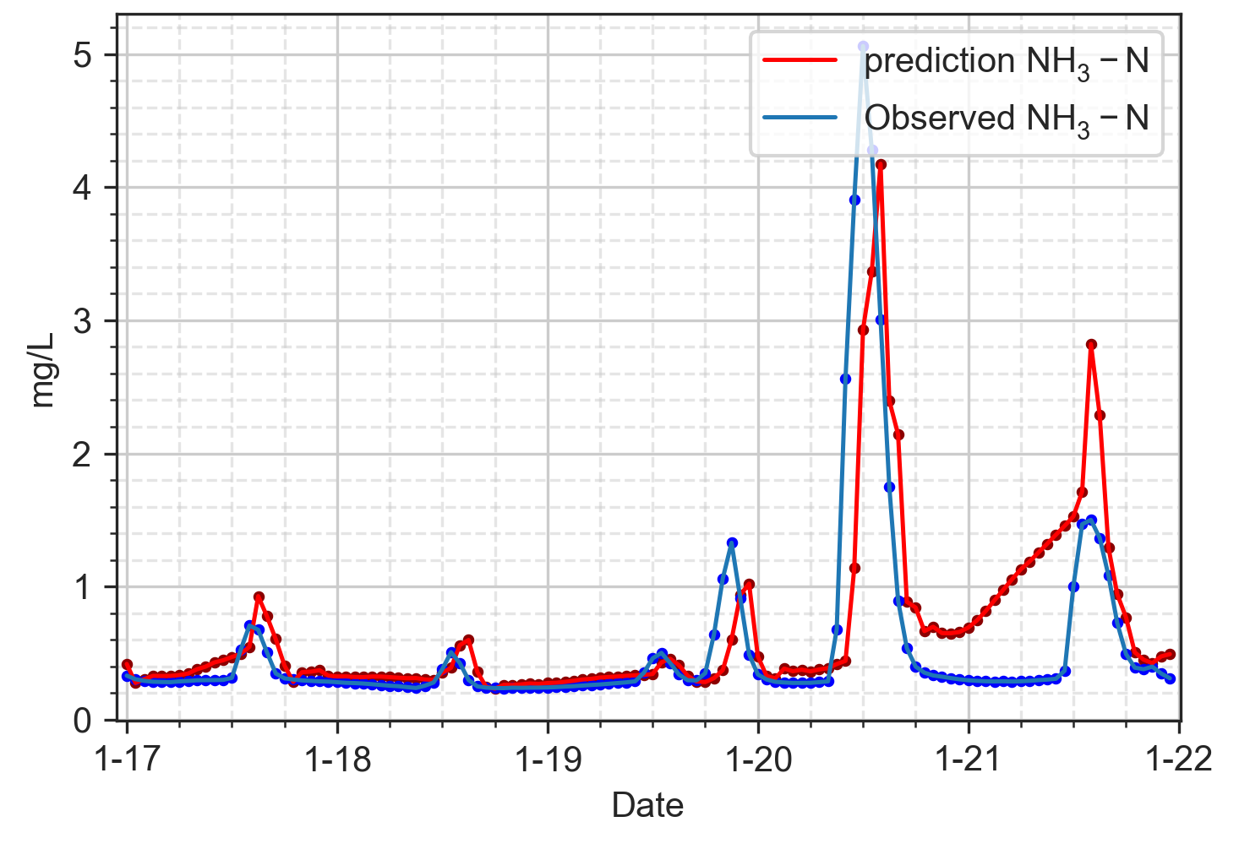
\includegraphics[width=\linewidth]{imgs/results/steps/nh3-lstm-1-fc2.png}
    \caption{LSTM-1-obs, MSE = 0.2916} \label{fig:nh3-lstm-1-fc2}
  \end{subfigure}\\
  \vspace{2em}
  \begin{subfigure}[t]{0.75\textwidth}
    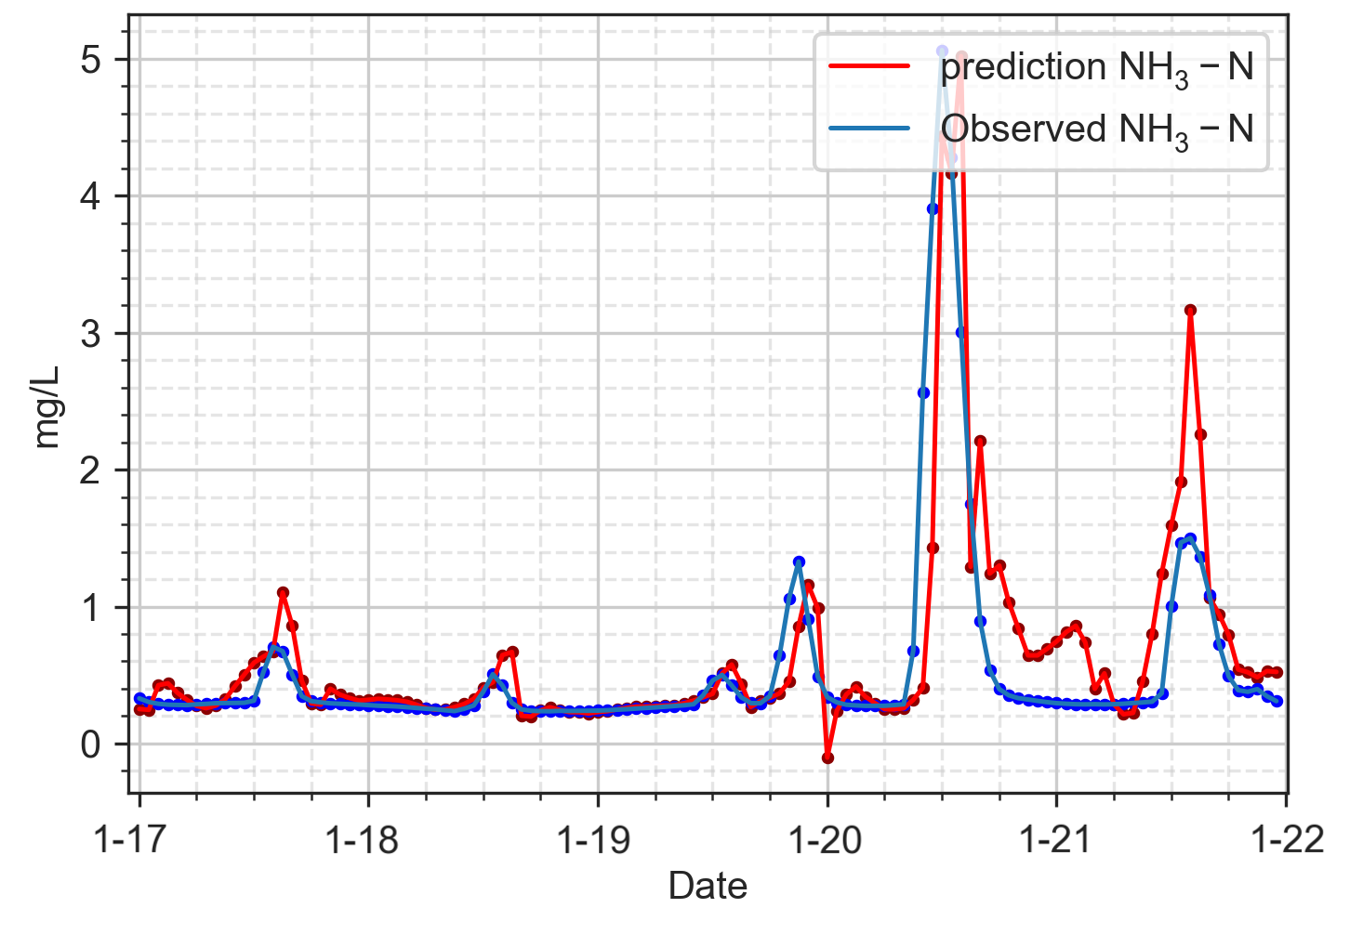
\includegraphics[width=\linewidth]{imgs/results/steps/nh3-lstm-4-fc2.png}
    \caption{LSTM-4-sg7, MSE = 0.2351} \label{fig:nh3-lstm-4-fc2}
  \end{subfigure}\\
\caption{Visualization of ammonia forecasting models at forecast horizon of two.} \label{fig:nh3-forecast-fc2}
\end{figure}

In forecasting ammonia concentration at a forecast horizon of three, although the MSE values of 0.7637 from LSTM-4-sg7 are lower than 0.8025 from LSTM-1-obs, the difference between the two model performances is negligible. For the LSTM-4-sg7 model, we observed ammonia concentrations lower than 0 mg/L were forecasted on 20 January. Both LSTM-4-sg7 and LSTM-1-obs models poorly forecasted the peak ammonia concentration of over 5.0 mg/L on 21 January, which is 3.0 mg/L higher than the actual ammonia concentration on the same day. The results suggest that even with the use of proposed model training methods, the capability of the model performance is still limited due to the limited size of the training dataset.

\begin{figure}[!ht]
  \centering
  \begin{subfigure}[t]{0.75\textwidth}
    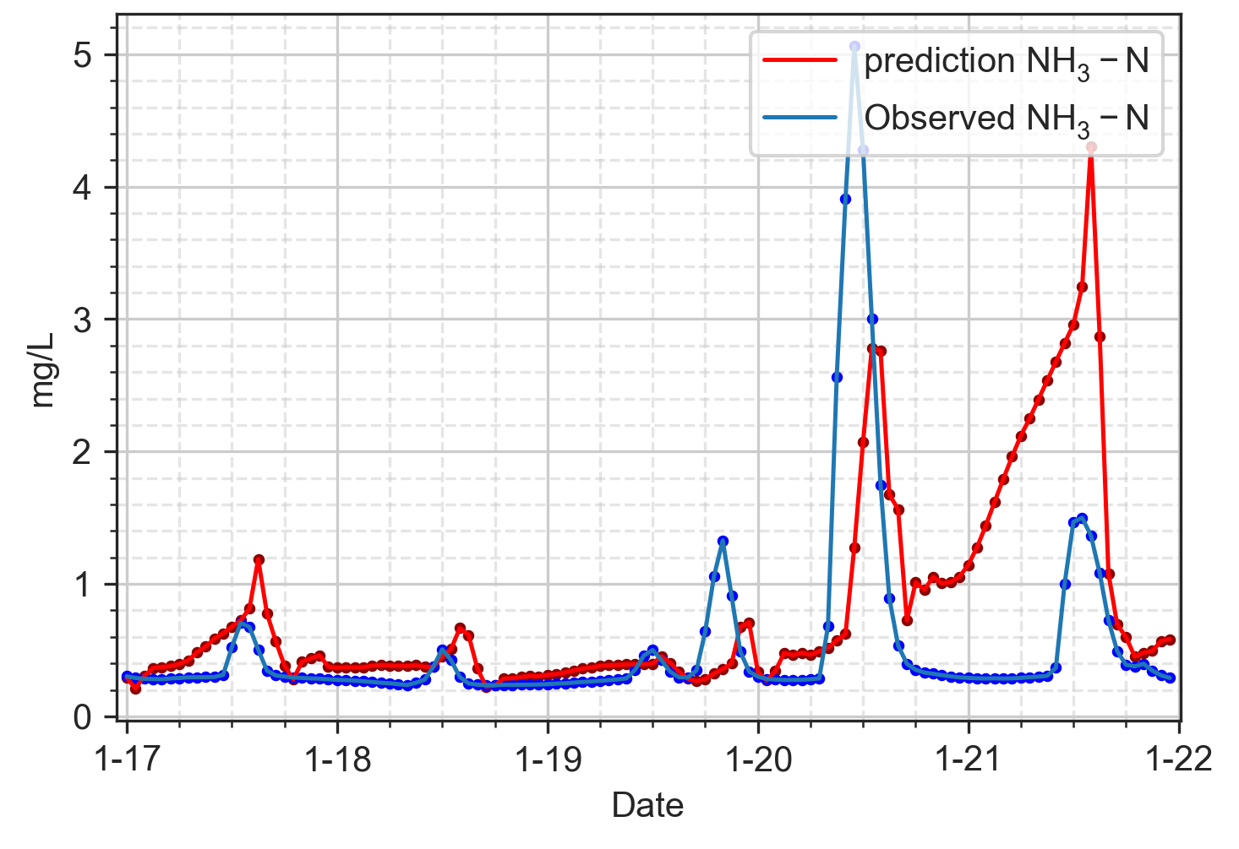
\includegraphics[width=\linewidth]{imgs/results/steps/nh3-lstm-1-fc3.png}
    \caption{LSTM-1-obs, MSE = 0.8025} \label{fig:nh3-lstm-1-fc3}
  \end{subfigure}\\
  \vspace{2em}
  \begin{subfigure}[t]{0.75\textwidth}
    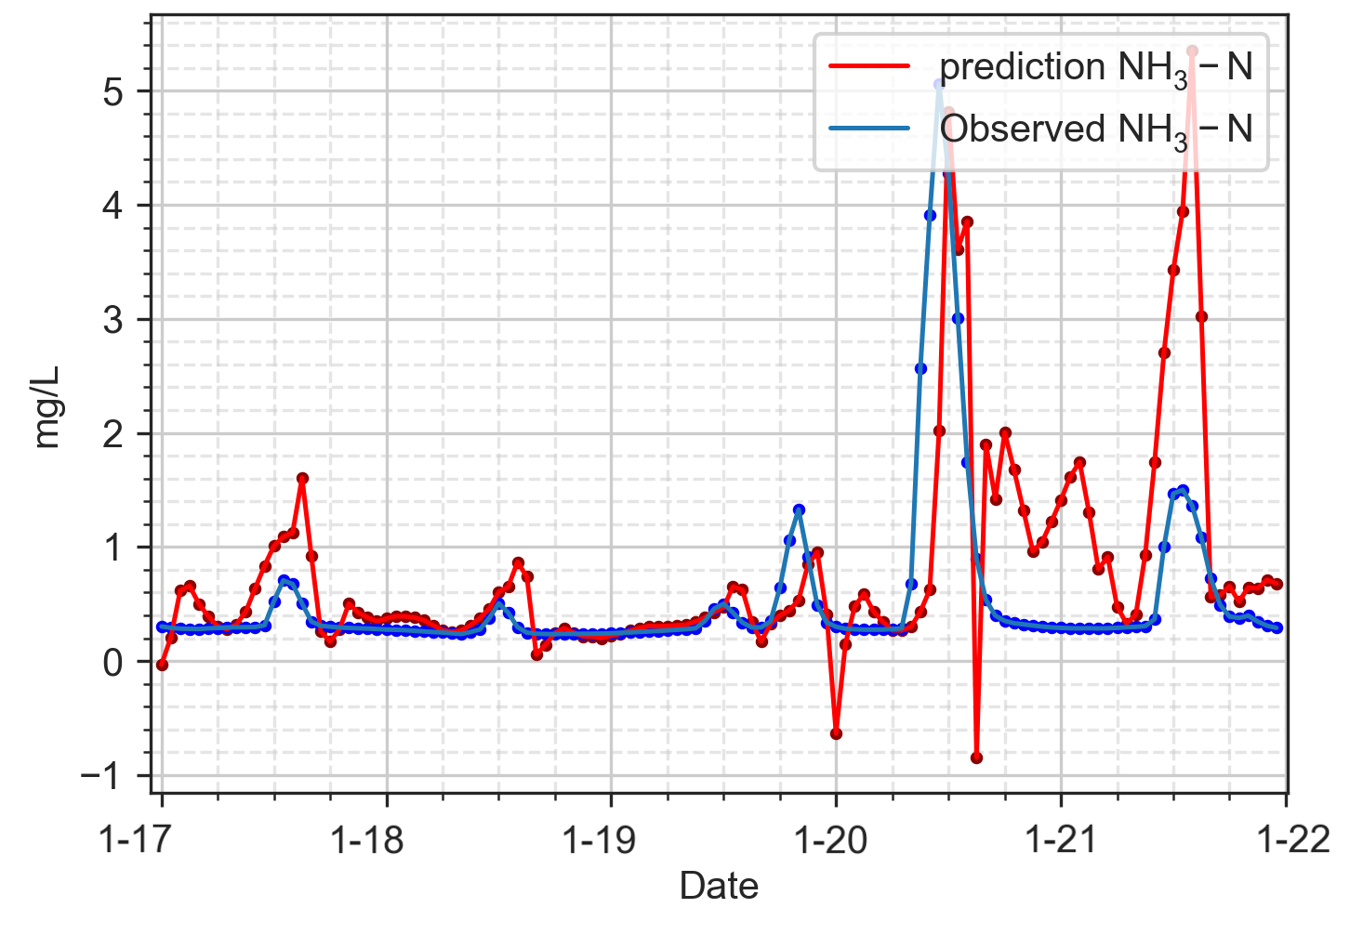
\includegraphics[width=\linewidth]{imgs/results/steps/nh3-lstm-4-fc3.png}
    \caption{LSTM-4-sg7, MSE = 0.7637} \label{fig:nh3-lstm-4-fc3}
  \end{subfigure}\\
\caption{Visualization of ammonia forecasting models at forecast horizon of three.} \label{fig:nh3-forecast-fc3}
\end{figure}

LSTM-1-obs and LSTM-3-sg9 models forecasted colour levels at a forecast horizon of one with good MSE values of 22.4922 and 17.5955. The errors between the actual and forecasted values are mostly less than 5 Hazen Units. On 18 January, the colour levels dropped to 80 Hazen Units, and both models forecasted colour levels with errours values of up to 5 Hazen Units and higher. Although on 22 January, the LSTM-3-sg9 model forecasted the colour level of 92 Hazen Units, which is 10 Hazen Units off from the actual values, the general model performance is satisfactory. 

\begin{figure}[!ht]
  \centering
  \begin{subfigure}[t]{0.7\textwidth}
    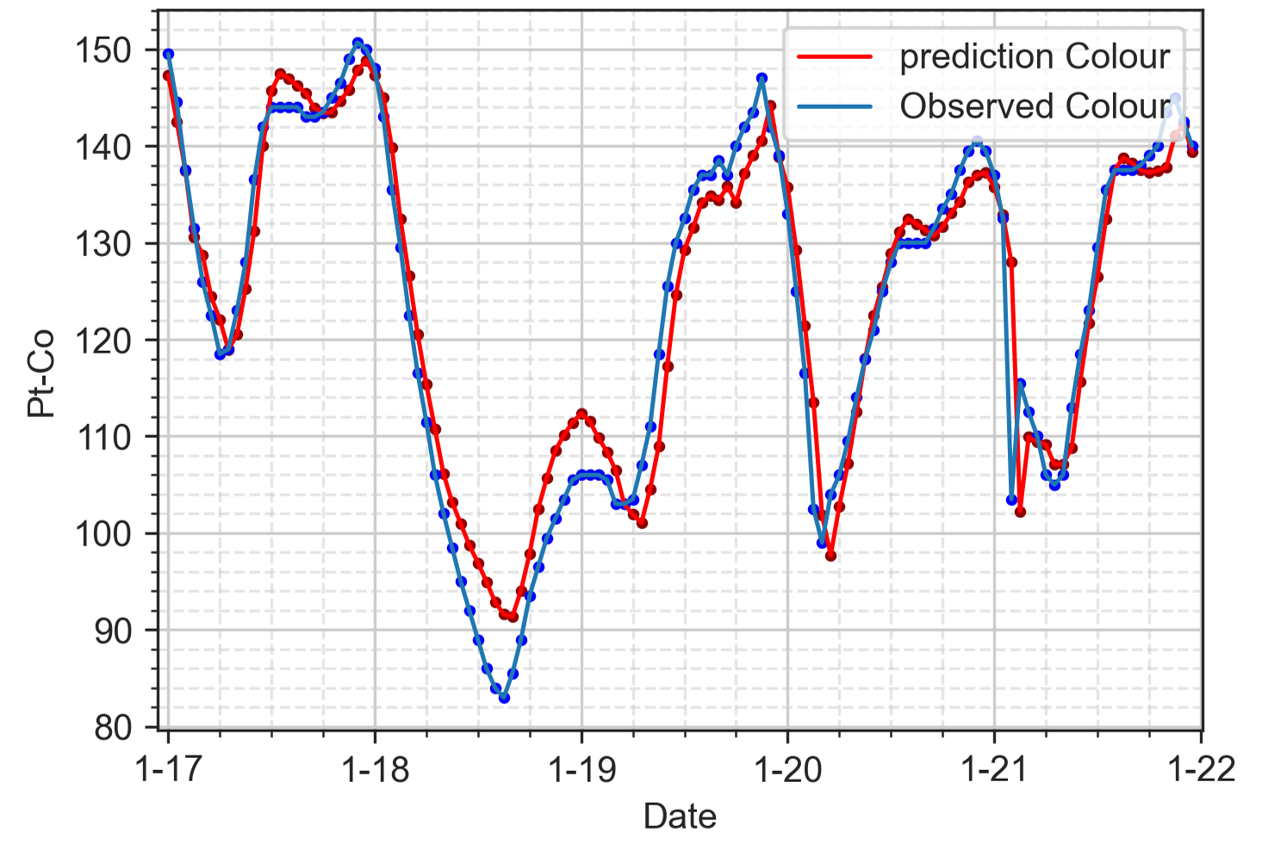
\includegraphics[width=\linewidth]{imgs/results/steps/colour-lstm-1-fc1.png}
    \caption{LSTM-1-obs, MSE = 22.4922} \label{fig:colour-lstm-1-fc1}
  \end{subfigure}\\
  \vspace{1em}
  \begin{subfigure}[t]{0.7\textwidth}
    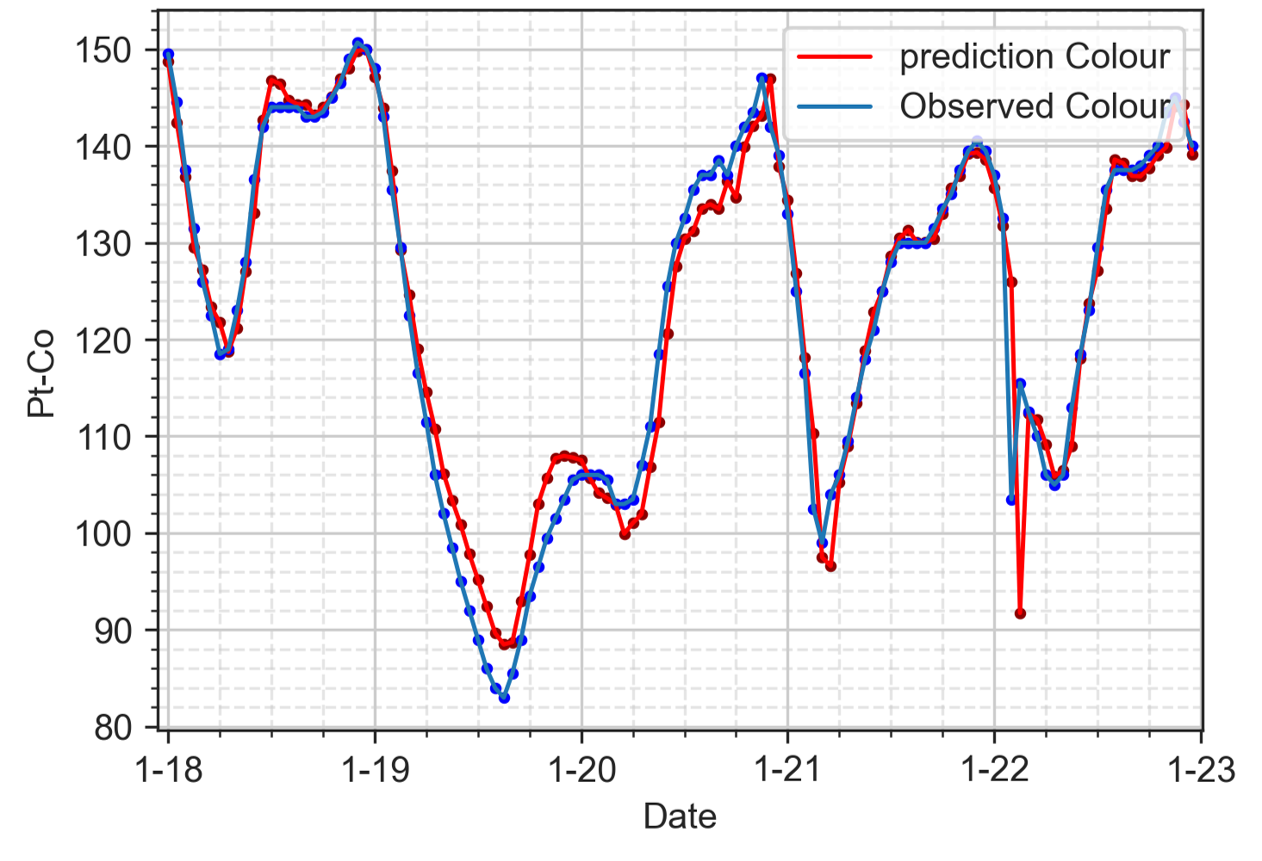
\includegraphics[width=\linewidth]{imgs/results/steps/colour-lstm-3-fc1.png}
    \caption{LSTM-3-sg9, MSE = 17.5955} \label{fig:colour-lstm-3-fc1}
  \end{subfigure}\\
\caption{Visualization of colour forecasting models at at forecast horizon of one.} \label{fig:colour-forecast-fc1}
\end{figure}

In forecasting colour levels at a forecast horizon of two, the MSE values of LSTM-1-obs and LSTM-3-sg9 increased from 22.4922 and 17.5955 to 62.6678 and 47.4252. The forecasting errors expanded from less than 5 Hazen Units on average to 10 Hazen Units. In Fig.~\ref{fig:colour-forecast-fc2}, LSTM-3-sg9 showed more reliable forecasting results compared to LSTM-1-obs by generating minor errors between the forecasted and actual values. However, the lowest forecasted colour level on 22 January has increased from 10 to 24 Hazen Unis, and we can see clearly that the models were getting less reliable in forecasting two hours into the future in forecasting colour levels. The cause of it can also be attributed to insufficient quantity of training dataset.

\begin{figure}[!ht]
  \centering
  \begin{subfigure}[t]{0.7\textwidth}
    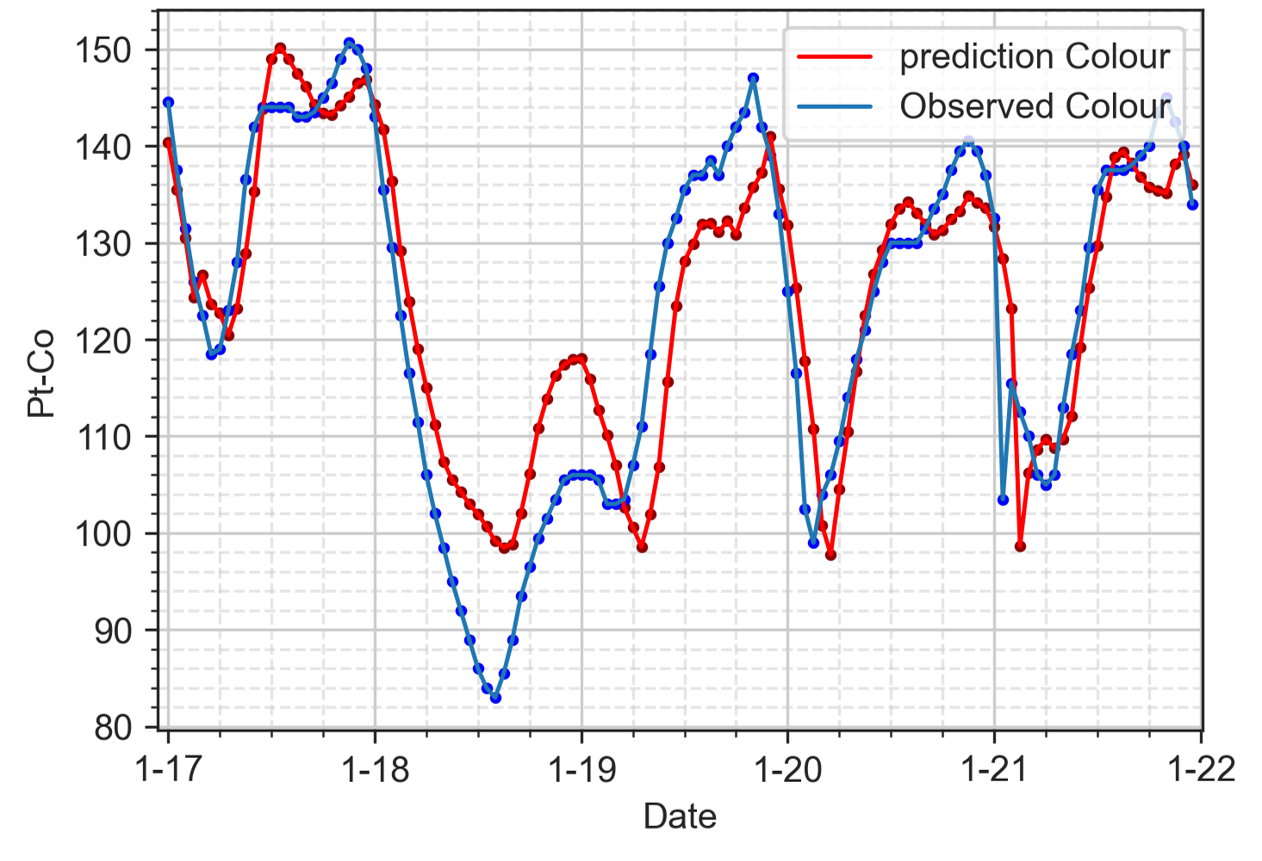
\includegraphics[width=\linewidth]{imgs/results/steps/colour-lstm-1-fc2.png}
    \caption{LSTM-1-obs, MSE = 62.6678} \label{fig:colour-lstm-1-fc2}
  \end{subfigure}\\
  \vspace{1em}
  \begin{subfigure}[t]{0.7\textwidth}
    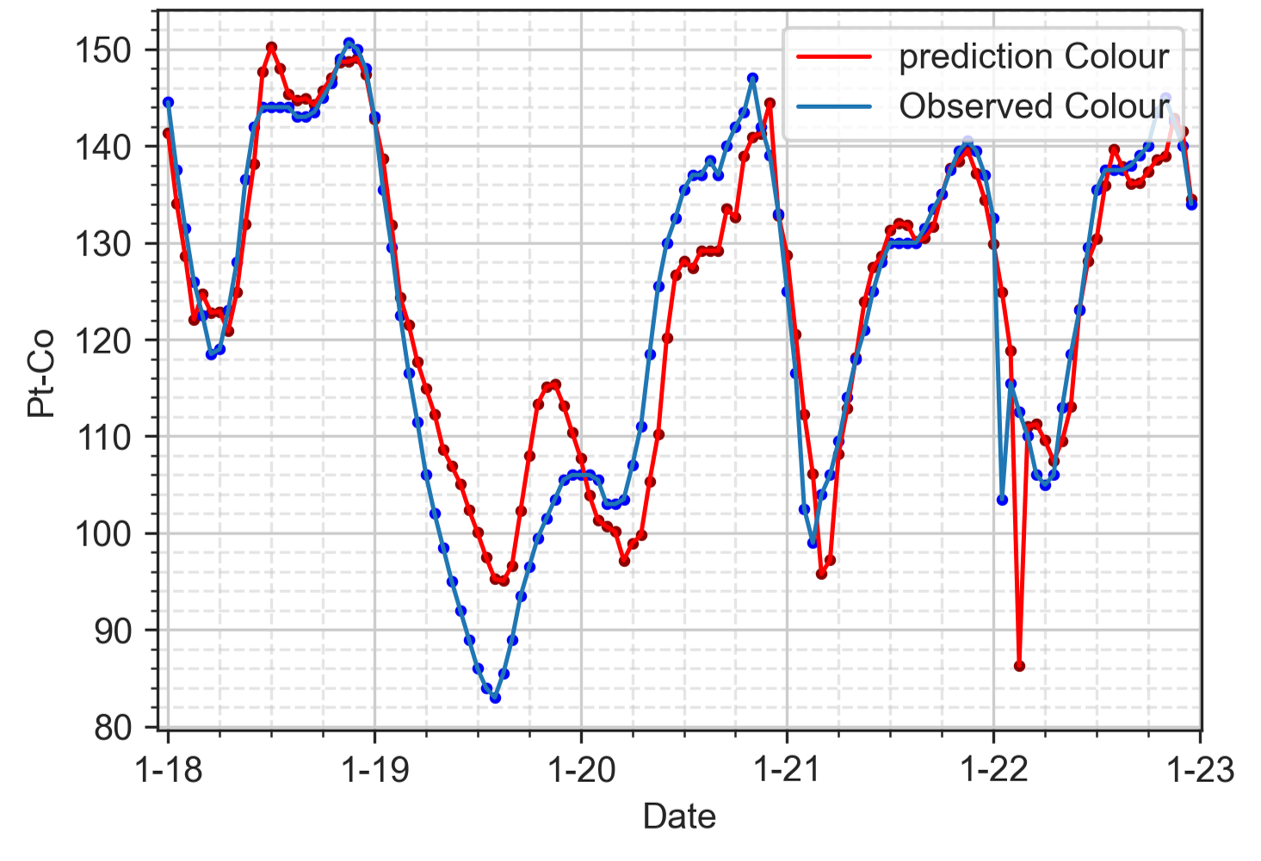
\includegraphics[width=\linewidth]{imgs/results/steps/colour-lstm-3-fc2.png}
    \caption{LSTM-3-sg9, MSE = 47.4252} \label{fig:colour-lstm-3-fc2}
  \end{subfigure}\\
\caption{Visualization of colour forecasting models at forecast horizon of two.} \label{fig:colour-forecast-fc2}
\end{figure}

In Fig.~\ref{fig:colour-forecast-fc3}, the MSE values of LSTM-1-obs and LSTM-3-sg9 have increased to 116.8928 and 103.4329 in forecasting colour levels at forecast horizons of three. We first noticed that both the models failed to forecast the lowest colour levels on 19 January. The significant drop in colour level can be a rare event in which the model did not learn how to react to such a change of colour levels from historical data. On the following days of 20 January, both the models underestimated the colour levels by forecasting up to 20 Hazen Units lower. The model performance deteriorated even faster than using ammonia forecasting models to forecast ammonia concentration at a forecast horizon of three. The results suggest that with much strong fluctuation of colour levels during the day, it is not reasonable to use colour forecasting models trained with only three input features to forecast three hours into the future.

\begin{figure}[!ht]
  \centering
  \begin{subfigure}[t]{0.7\textwidth}
    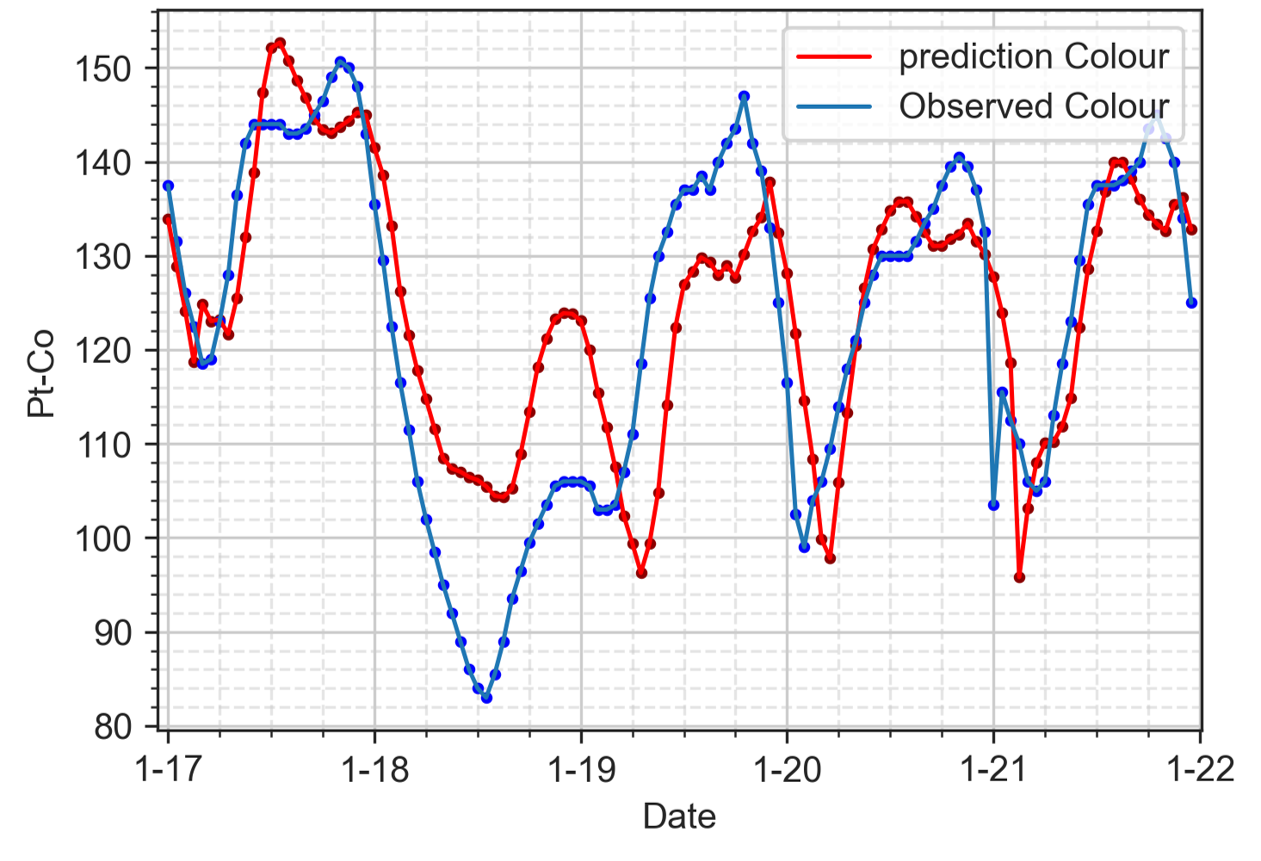
\includegraphics[width=\linewidth]{imgs/results/steps/colour-lstm-1-fc3.png}
    \caption{LSTM-1-obs, MSE = 116.8928} \label{fig:colour-lstm-1-fc3}
  \end{subfigure}\\
  \vspace{1em}
  \begin{subfigure}[t]{0.7\textwidth}
    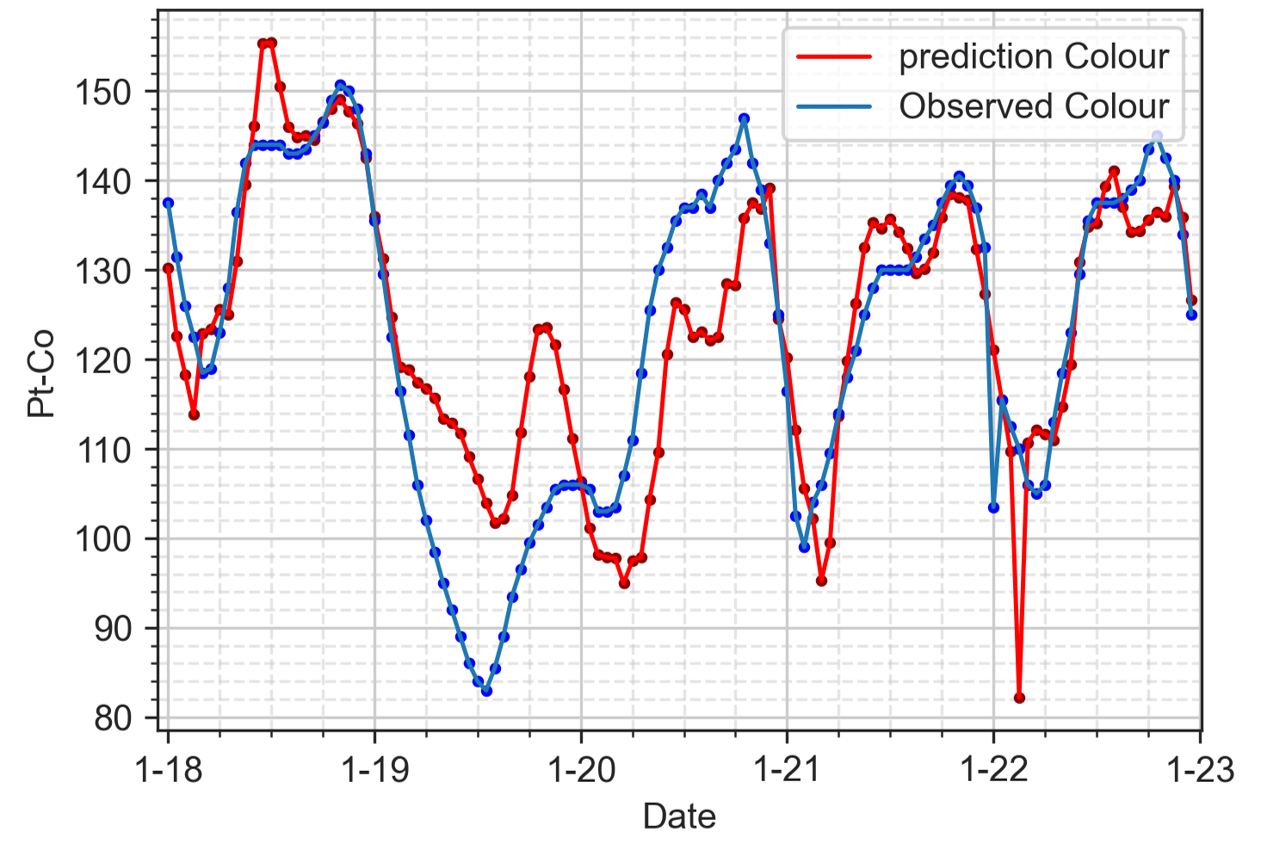
\includegraphics[width=\linewidth]{imgs/results/steps/colour-lstm-3-fc3.png}
    \caption{LSTM-3-sg9, MSE = 103.4329} \label{fig:colour-lstm-3-fc3}
  \end{subfigure}\\
\caption{Visualization of colour forecasting models at forecast horizon of three.} \label{fig:colour-forecast-fc3}
\end{figure}
